\documentclass[colorlinks,11pt,a4paper,normalphoto,withhyper,ragged2e]{altareport}


%%%%%%%%%%%%%%%%%%%%%%%%%%%%%%%%%%%%%%%%%%%
%%%%%%%%%% DEFAULT PACKAGES & SETTINGS %%%%%%%%%%
\usepackage[utf8]{inputenc}
\usepackage{setspace} %1.5 line spacing
\usepackage{notoccite} %% Citation numbering
\usepackage{lscape} %% Landscape table
\usepackage{caption} %% Adds a newline in the table caption

%% The paracol package lets you typeset columns of text in parallel
\usepackage{paracol}
\usepackage[none]{hyphenat}

%% Document and Theme Fonts
\usepackage[T1]{fontenc}
\usepackage{paratype}
\usepackage[defaultsans]{lato}
%\usepackage[sfdefault,light,condensed]{roboto}
%\usepackage[rm]{roboto}
%\usepackage[defaultsans]{lato}
%\usepackage{sourcesanspro}
%\usepackage[rm]{merriweather}

\captionsetup{font=footnotesize}

\setlength{\intextsep}{4pt} % Set defualt spacing around floats

%%%%%%%%%%%%%%%%%%%%%%%%%%%%%%%%%%%%%%%%%%%


%%%%%%%%%%%%%%%%%%%%%%%%%%%%%%%%%%%%%%%%%%%
%%%%%%%%%% THEMES %%%%%%%%%%

%% Standard theme options are below, leave blank for B&W / no colours (BoringDefault). Note the theme will be set to default if you enter a non-exsistant theme name.
\SetTheme{UNIBS}
%% UNIBS
%% UNILIM
%% PastelBlue
%% GreenAndGold
%% Purple
%% PastelRed
%% BoringDefault (Leave blank / enter anything not found above)

%%%%%%%%%%%%%%%%%%%%%%%%%%%%%%%%%%%%%%%%%%%






%%%%%%%%%%%%%%%%%%%%%%%%%%%%%%%%%%%%%%%%%%%
%%%%%%%%%% DOCUMENT SPECIFIC PACKAGES %%%%%%%%%%

\usepackage{amssymb}
\usepackage{amsfonts}
\usepackage{mathtools}

\usepackage{pythontex} % Run python code in this latex doc

%%%%%%%%% Karnaugh Map Package & Settings %%%%%%%%%
\usepackage[export]{adjustbox}

\usetikzlibrary{matrix,calc}
\usepackage{karnaugh-map}

\colorlet{LightRed}{red!60!}
\colorlet{LightBlue}{blue!60!}
\colorlet{LightYellow}{yellow!60!}
\colorlet{LightGreen}{green!60!}
\colorlet{LightOrange}{orange!60!}

%%%%%%%%% MATLAB Language Settings %%%%%%%%%
\usepackage[numbered,framed]{matlab-prettifier} % To add code listings from matlab
\lstMakeShortInline[style=Matlab-editor]" %% This makes " an escape character to write in matlab editor font


%%%%% Settings for python pgf graphs %%%%%
\usepackage{pgfplots}
\usetikzlibrary{arrows.meta}

\pgfplotsset{compat=newest,
    width=6cm,
    height=3cm,
    scale only axis=true,
    max space between ticks=25pt,
    try min ticks=5,
    every axis/.style={
        axis y line=left,
        axis x line=bottom,
        axis line style={thick,->,>=latex, shorten >=-.4cm}
    },
    every axis plot/.append style={thick},
    tick style={black, thick}
}
\tikzset{
    semithick/.style={line width=0.8pt},
}

\usepgfplotslibrary{groupplots}
\usepgfplotslibrary{dateplot}


% Reduce space around captions
% \captionsetup{aboveskip=5pt, belowskip=5pt}
%%%%%%%%%%%%%%%%%%%%%%%%%%%%%%%%%%%%%%%%%%%




%%%%%%%%%%%%%%%%%%%%%%%%%%%%%%%%%%%%%%%%%%%
%%%%%%%%%% USEFUL SETTINGS %%%%%%%%%%
%% Change some font sizes, this will override the defaults
\renewcommand{\ReportTitleFont}{\Huge\rmfamily\bfseries} %% Title Page - Main Title
\renewcommand{\ReportSubTitleFont}{\huge\bfseries} %% Title Page - Sub-Title
\renewcommand{\ReportSectionFont}{\LARGE\rmfamily\bfseries} %% Section Title
\renewcommand{\ReportSubSectionFont}{\large\bfseries} %% SubSection Title
\renewcommand{\FootNoteFont}{\footnotesize} %% Footnotes and Header/Footer

%% Change the bullets for itemize and rating marker
\renewcommand{\itemmarker}{{\small\textbullet}}
\renewcommand{\ratingmarker}{\faCircle}

%% Change the page layout
\geometry{left=1.5cm,right=1.5cm,top=3cm,bottom=3cm,columnsep=8mm}
\onehalfspace   % 1.5 line spacing

\definecolor{CommentGreen}{HTML}{228B22}
%%%%%%%%%%%%%%%%%%%%%%%%%%%%%%%%%%%%%%%%%%%




%%%%%%%%%%%%%%%%%%%%%%%%%%%%%%%%%%%%%%%%%%%
%\include{references.bib}

%%%%%%%%%% TITLE PAGE INFO %%%%%%%%%%
\ReportTitle{Wireless Systems Lab}
\SubTitle{Exercise One: Dipole and Monopole (CST)}
\Author{Andrew Simon Wilson}
\ReportDate{\today}
\FacultyOrLocation{EMIMEO Programme}
\ModCoord{Prof. Daniele Modotto}

%%%%%%%%%%%%%%%%%%%%%%%%%%%%%%%%%%%%%%%%%%%


\newcommand*\circled[1]{\tikz[baseline=(char.base)]{
            \node[shape=circle,draw,inner sep=0.5pt] (char) {#1};}}


\begin{document}

\MakeReportTitlePage


%%%%% CONTENTS %%%%%
\pagenumbering{roman} % Start roman numbering
\setcounter{page}{1}


%%%%%%%%%% YOUR NAME, PROFESSION, PORTRAIT, CONTACT INFO, SOCIAL MEDIA ETC. %%%%%%%%%%
\name{Andrew Simon Wilson, BEng}
\tagline{Post-graduate Masters Student, Erasmus Mundus JMD - EMIMEO Programme}

\personalinfo{
  \email{andrew.s.wilson@protonmail.com}
  \linkedin{andrew-simon-wilson} 
  \github{AS-Wilson}
  \phone{+44 7930 560 383}
}

%% You can add multiple photos on the left or right
% \photoR{3cm}{Images/a-wilson-potrait.jpg}
% \photoL{3cm}{Yacht_High,Suitcase_High}


\section*{Author Details}
\makeauthordetails

%% Table of contents print level -1: part, 0: chapter, 1: section, 2:sub-section, 3:sub-sub-section, etc.
\setcounter{tocdepth}{2} 
\tableofcontents %% Prints a list of all sections based on the above command
%\listoffigures %% Prints a list of all figures in the report
%\listoftables %% Prints a list of all tables in the report



%%%%%% INTRO %%%%%
%\section*{Introduction}
%Here is and example how you cite throughout the document\cite{JenningsWilson2021}, the default bibliography format is IEEE Transactions.
%\newpage



%%%%%%%%%% DOCUMENT CONTENT BEGINS HERE %%%%%%%%%%

\pagenumbering{arabic} % Start document numbering - roman numbering

\newpage

\section{Half-Wavelength Dipole Antenna}
My Matriculation number is 740239 (an odd number) and as such my central frequency is 1.5GHz (it was originally 5.58GHz, but as the student licence cannot process the mesh density required for that frequency a new, alternative was presented by Prof. Modotto).

\subsection{Question One}
First I used CST Studio's built in wavelength calculator to obtain an initial value for the wavelength of 199.86mm and made this a parameter for the design of the dipole. I obtained an initial set of S(1,1) parameters as shown on the left in Figure \ref{fig:hw_s11_params_init_sweeps}. Afterwards I ran two parameter sweeping simulations changing the value of lambda broadly initially, then changing the calculate more precisely; the S(1,1) parameters for these sweeps are shown in the middle and the left of Figure \ref{fig:hw_s11_params_init_sweeps}.

\begin{figure}[h]
	\centering
	\hspace{\fill}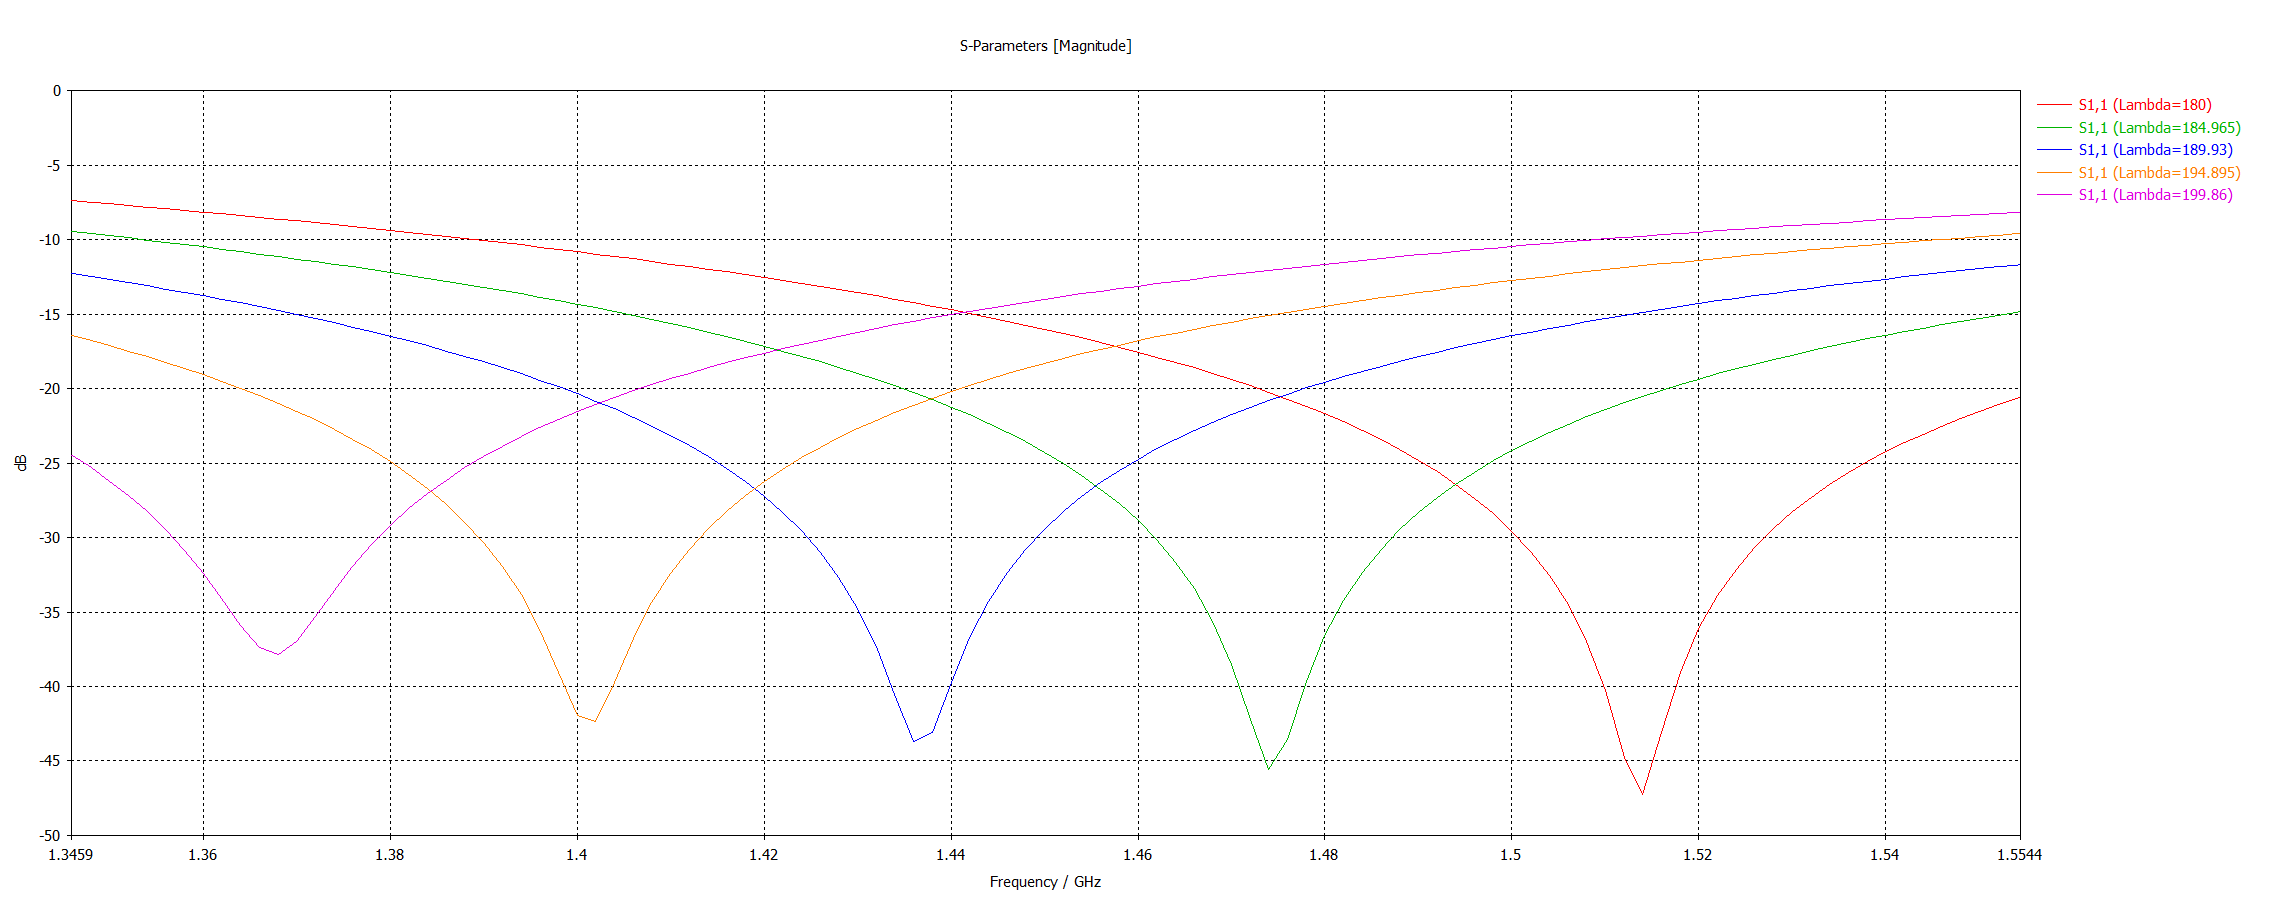
\includegraphics[width=9cm,valign=c]{Images/hw-lambda-sweep-broad-S1,1.png}\hspace{\fill}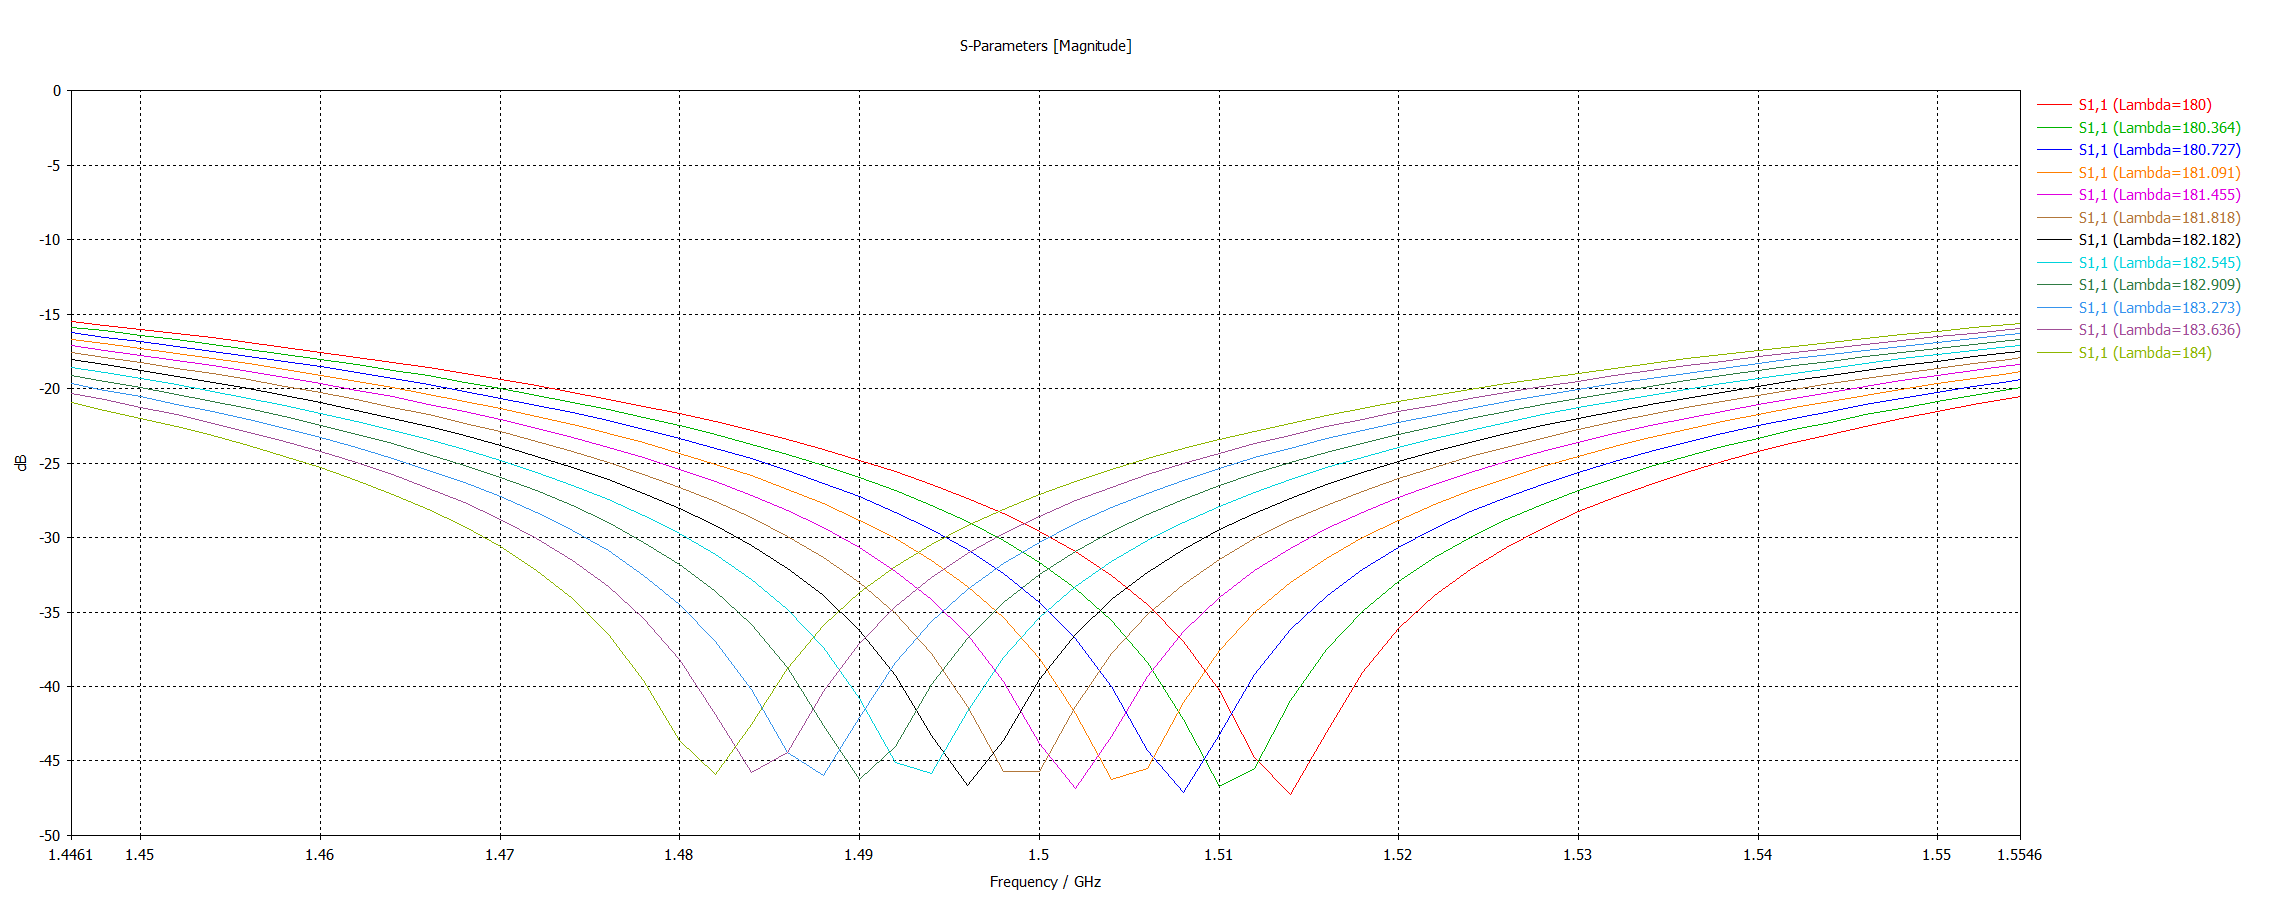
\includegraphics[width=9cm,valign=c]{Images/hw-lambda-sweep-narrow-S1,1.png}\hspace{\fill}
	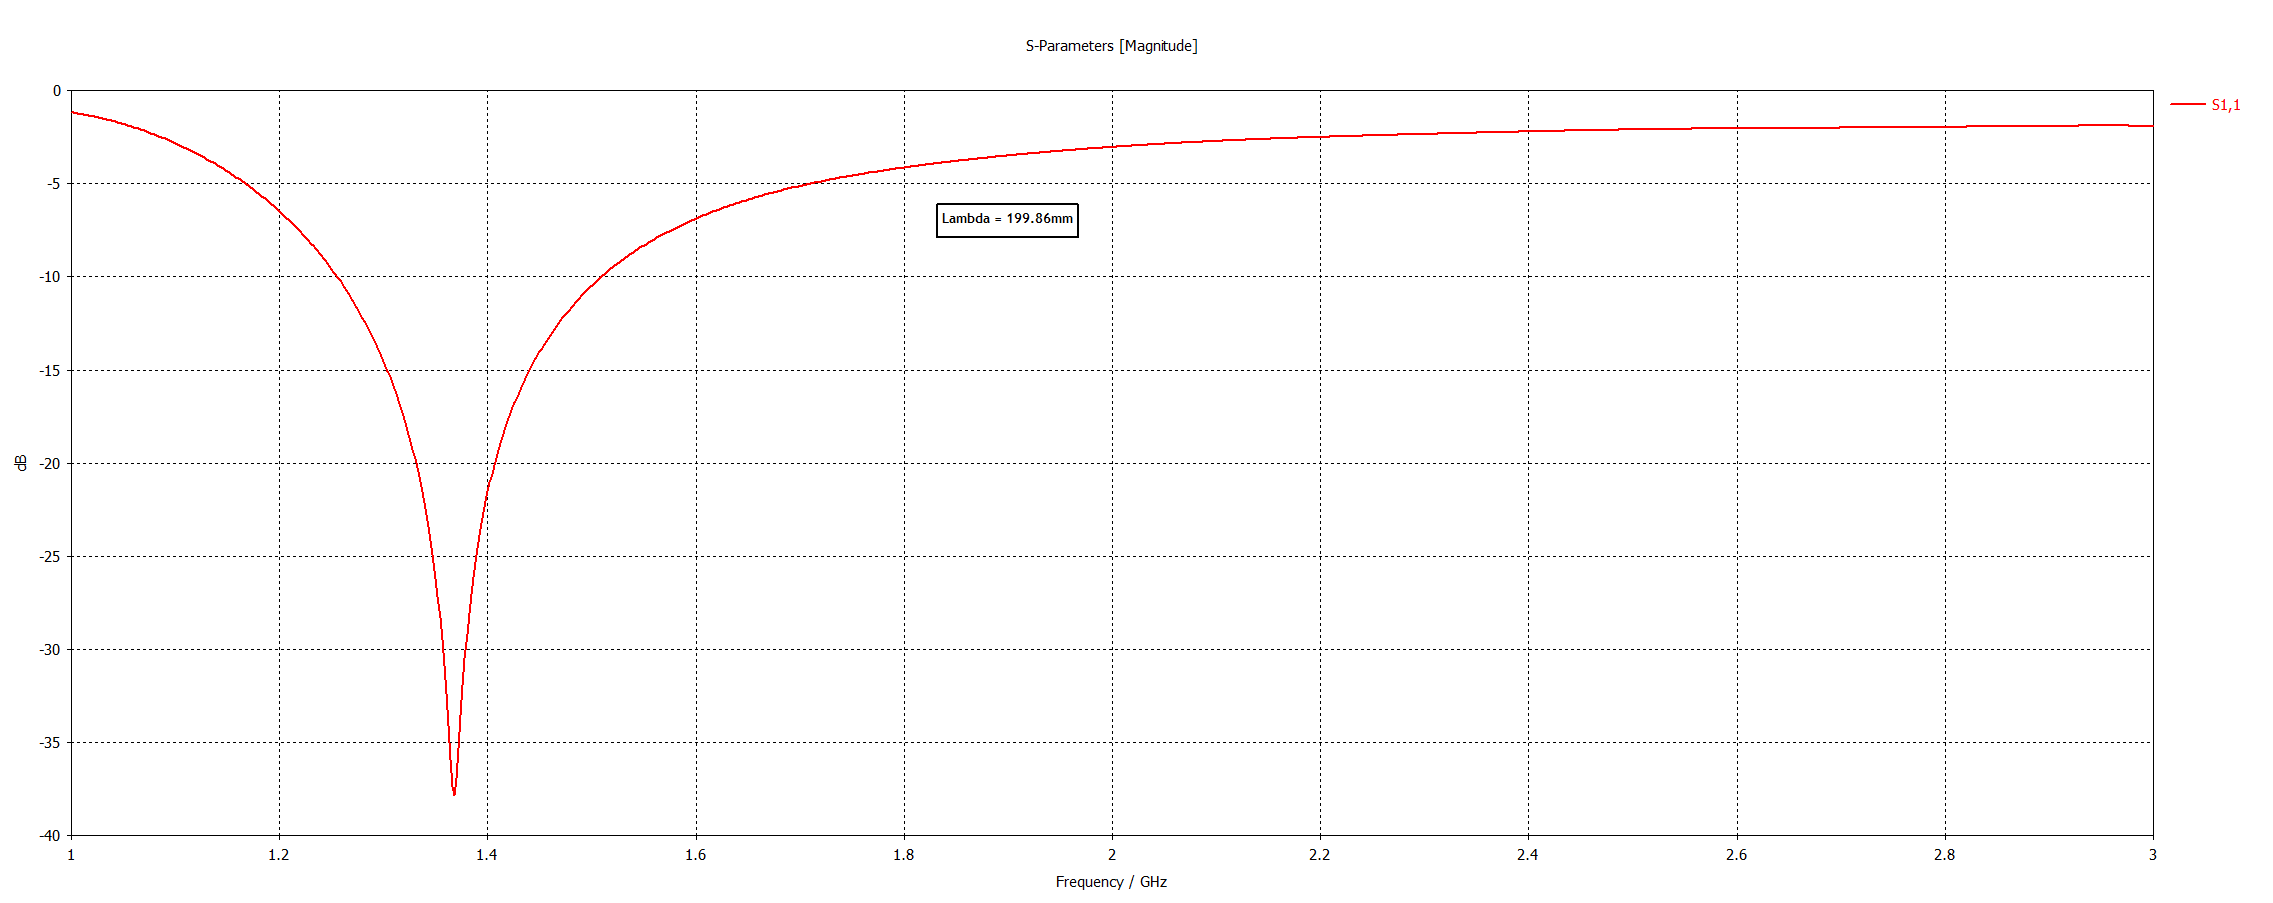
\includegraphics[width=12cm,valign=c]{Images/hw-lambda-199.86-S1,1.png}
	\caption{S1,1 Parameters for initially calculated wavelength (bottom) and the broad and narrow parameter sweeps (top left and right respectively)}  %% Caption for your figure
	\label{fig:hw_s11_params_init_sweeps}
\end{figure}

Using the parameter sweeps I obtained the final value for lambda as 181.75mm this subsequently allowed me to set the dimensions as shown on the left in Figure \ref{fig:hw_s11_dimesions_final} and simulated the S(1,1) results, again in Figure \ref{fig:hw_s11_dimesions_final}.

\begin{figure}[h!]
	\centering
	\hspace{\fill}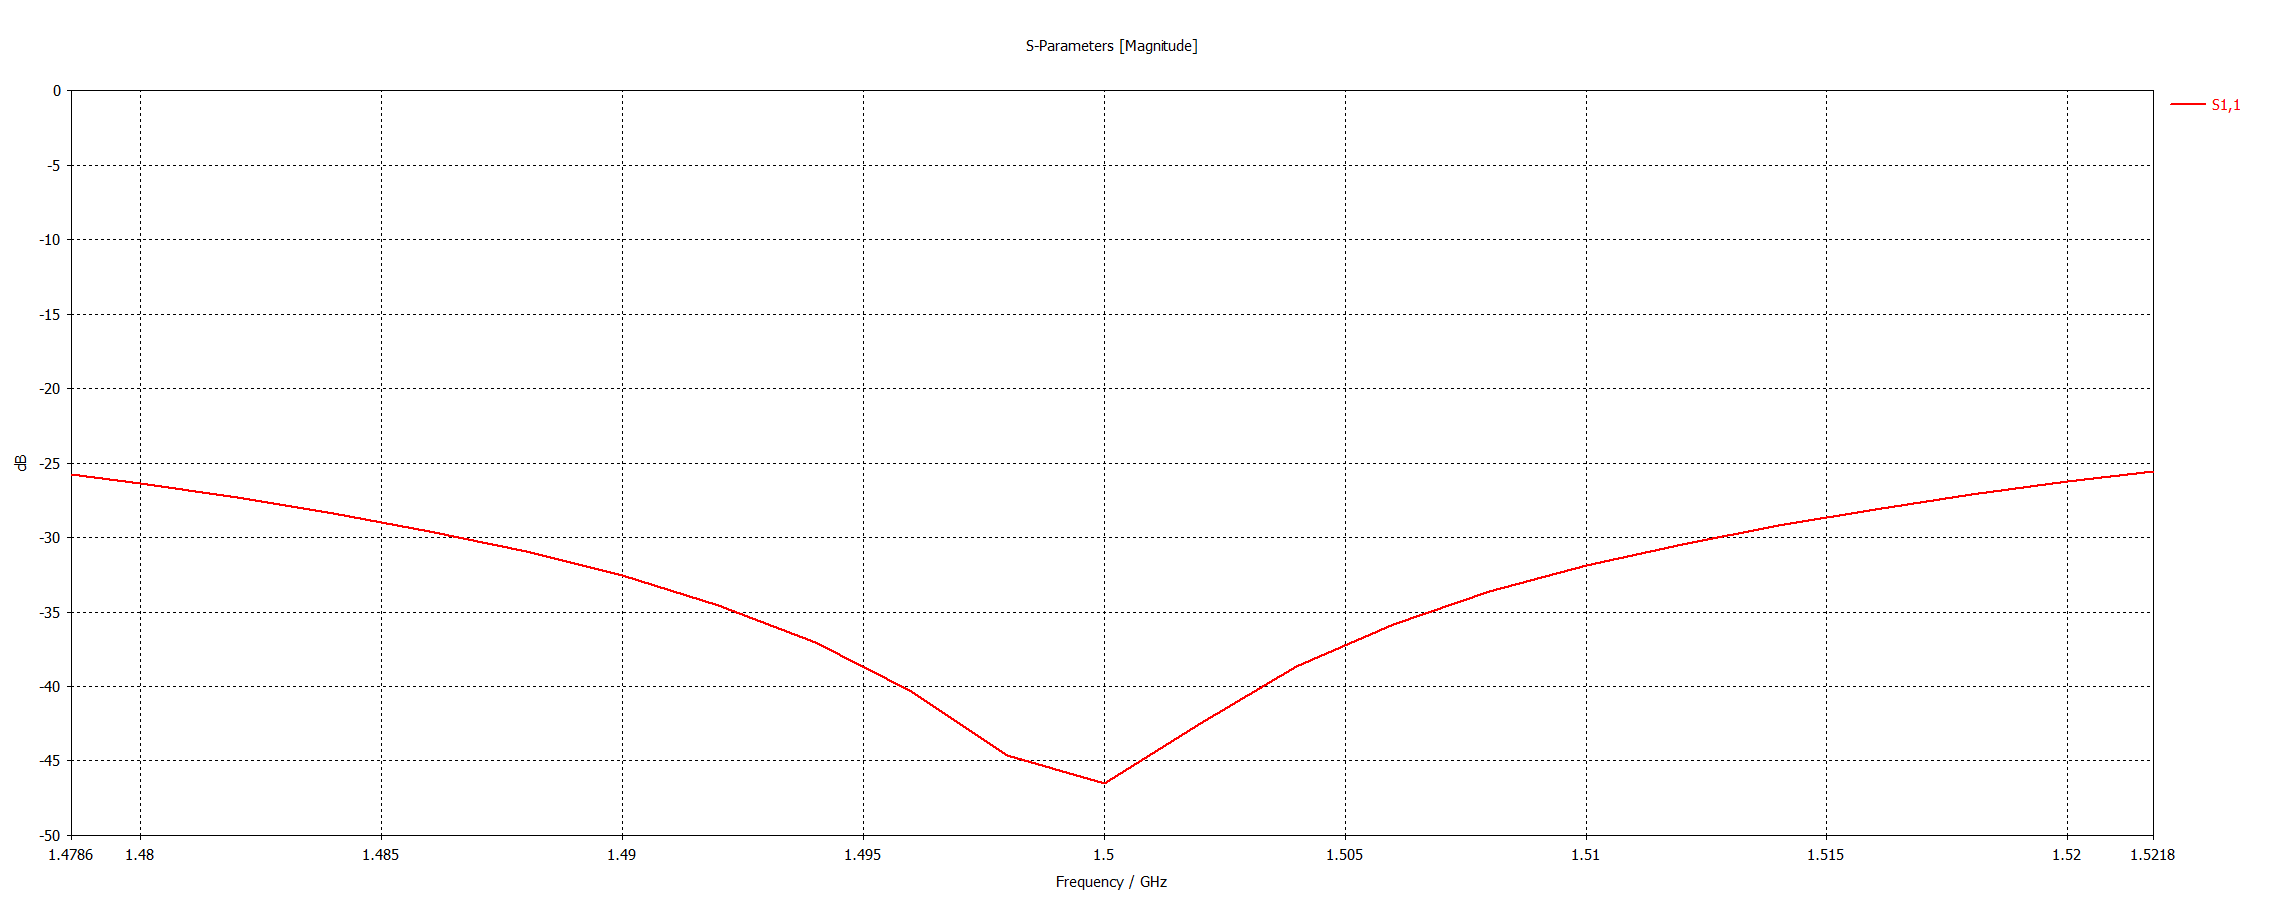
\includegraphics[width=10cm,valign=c]{Images/hw-lambda-181.75-S1,1.png}\hspace{\fill}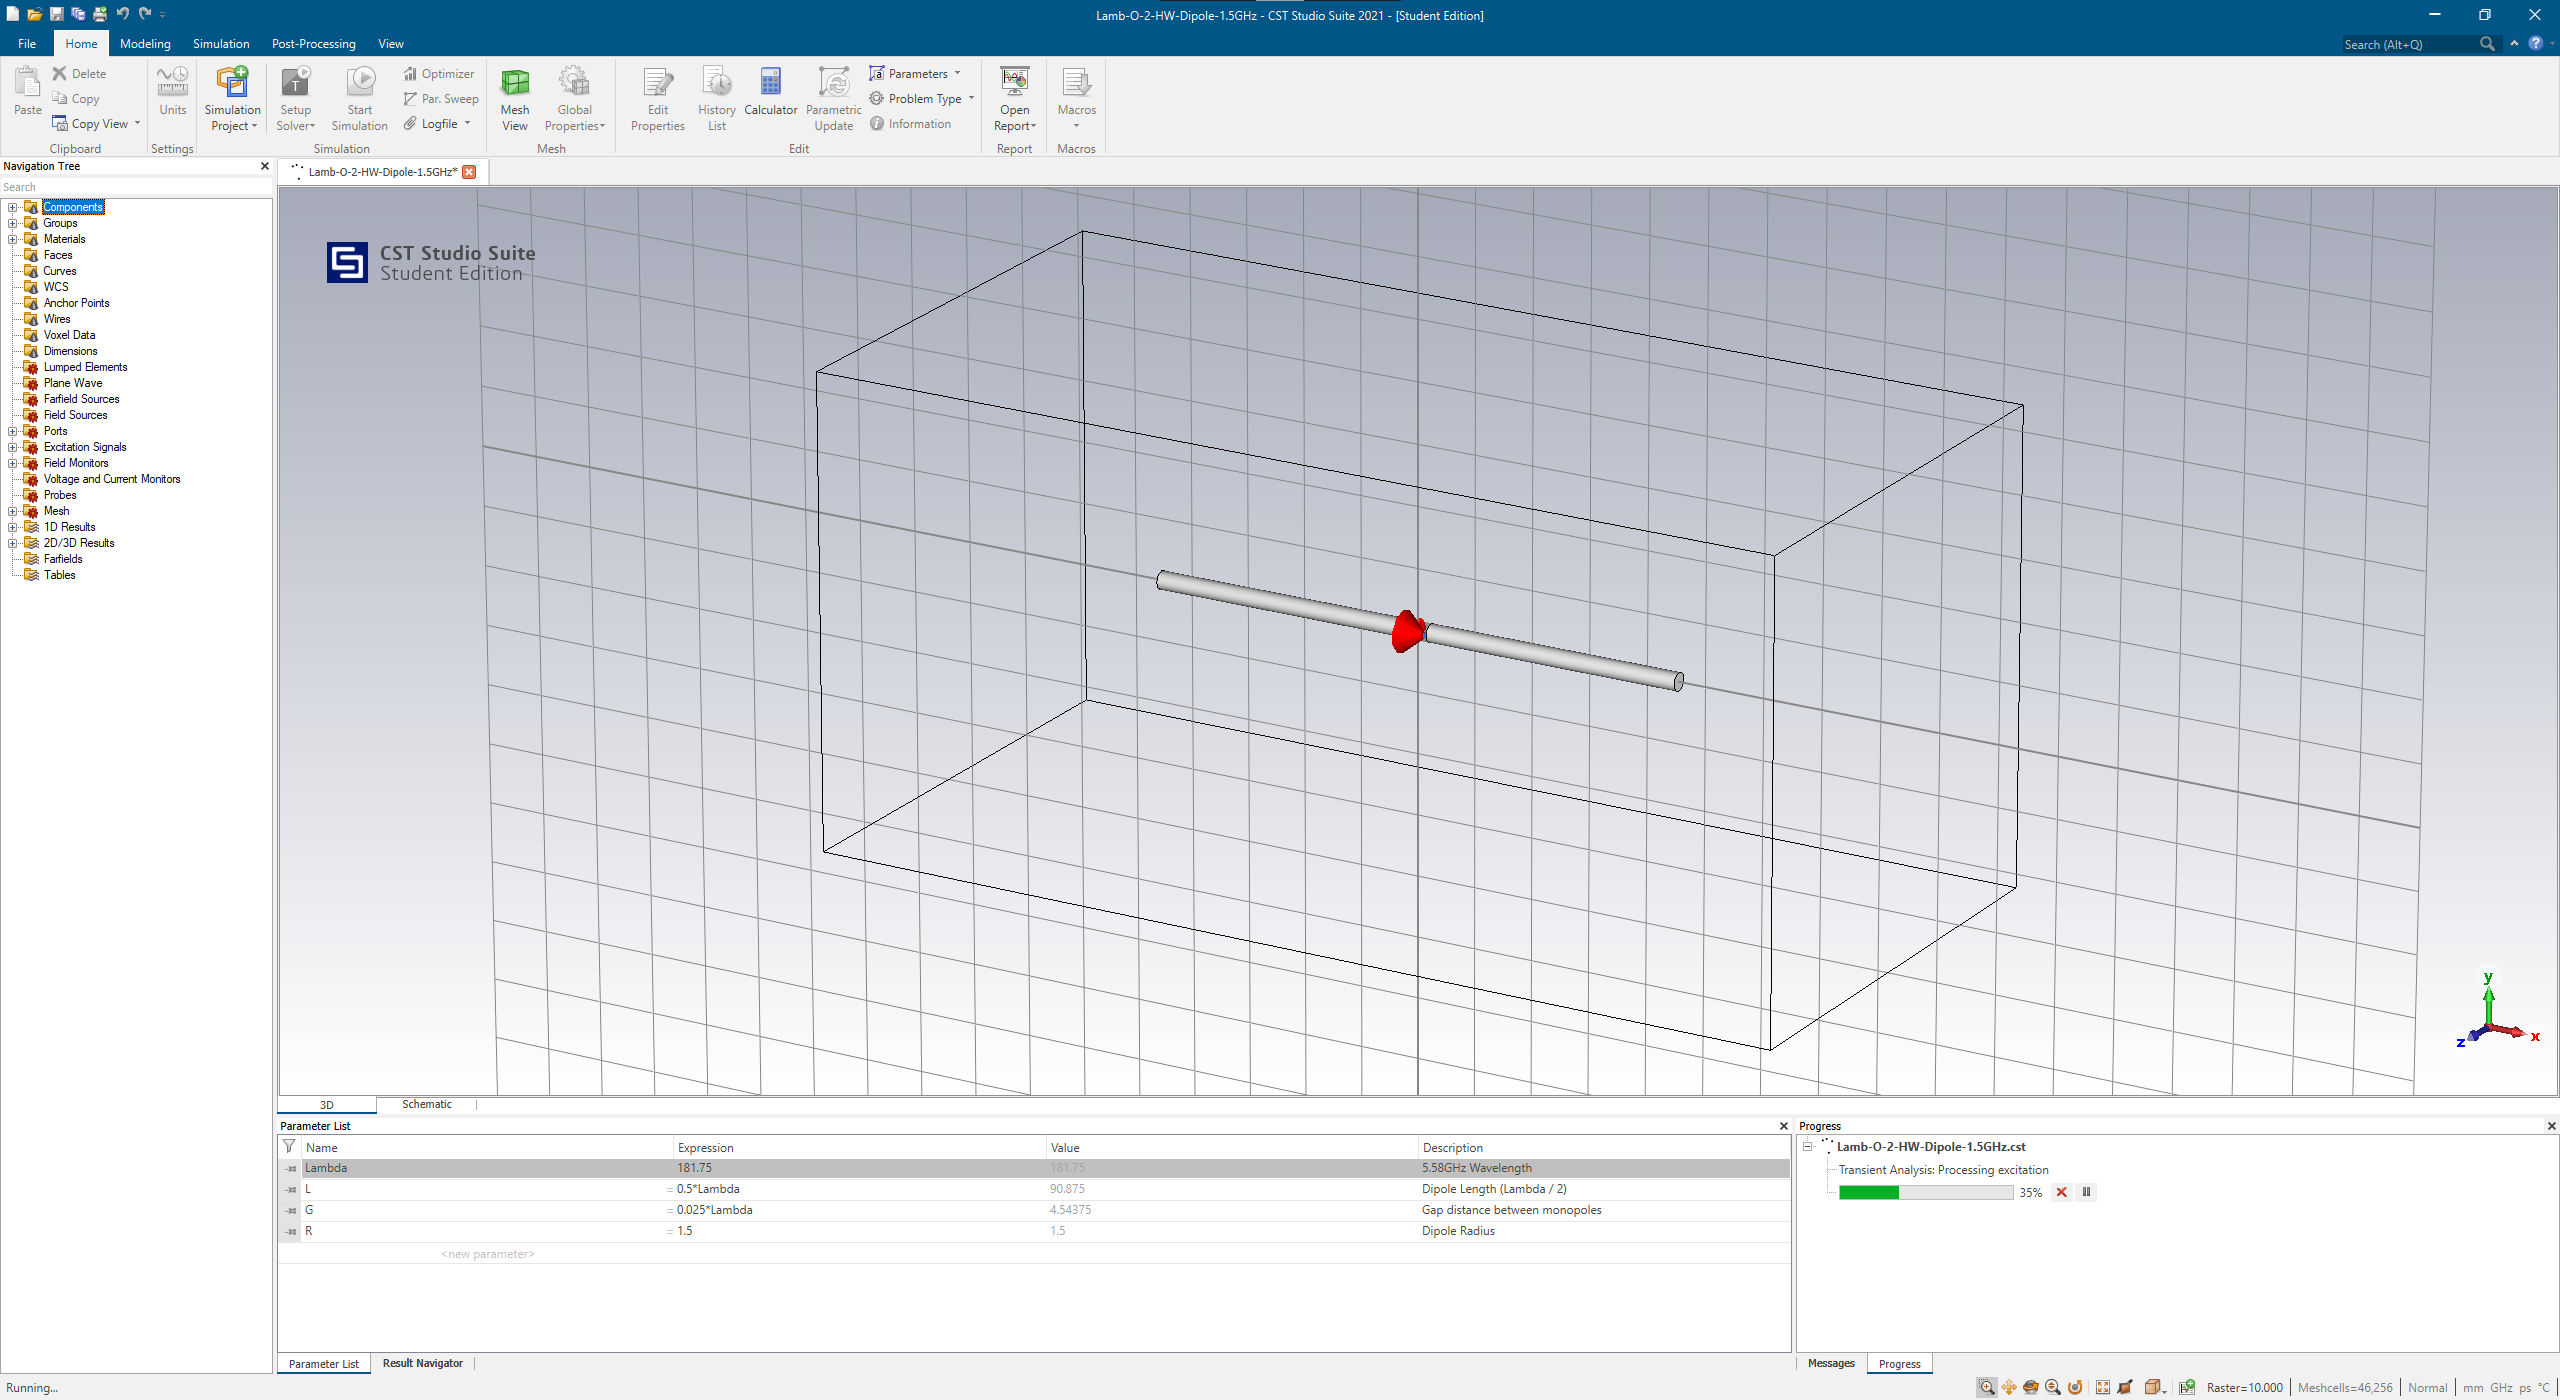
\includegraphics[width=8cm,valign=c]{Images/hw-final-dimens.png}\hspace{\fill}
	\caption{The final S(1,1) parameters (left) and the final dimensions and design of the dipole (right)}
	\label{fig:hw_s11_dimesions_final}
\end{figure}




\subsection{Question Two}

Plotting the E and H fields shows, as one would expect from a half wave dipole, the E-field in the X-Y plane is shown in Figure \ref{fig:hw_e_field_xy}, one can see that the electric field is moving in the same direction as the port excitation, with the left hand side acting as the cathode of the antenna and the right hand side the anode. Additionally one can see that the E-field is strongest at the edges of the antenna. \linebreak

\begin{figure}[h]
	\centering
	\hspace{\fill}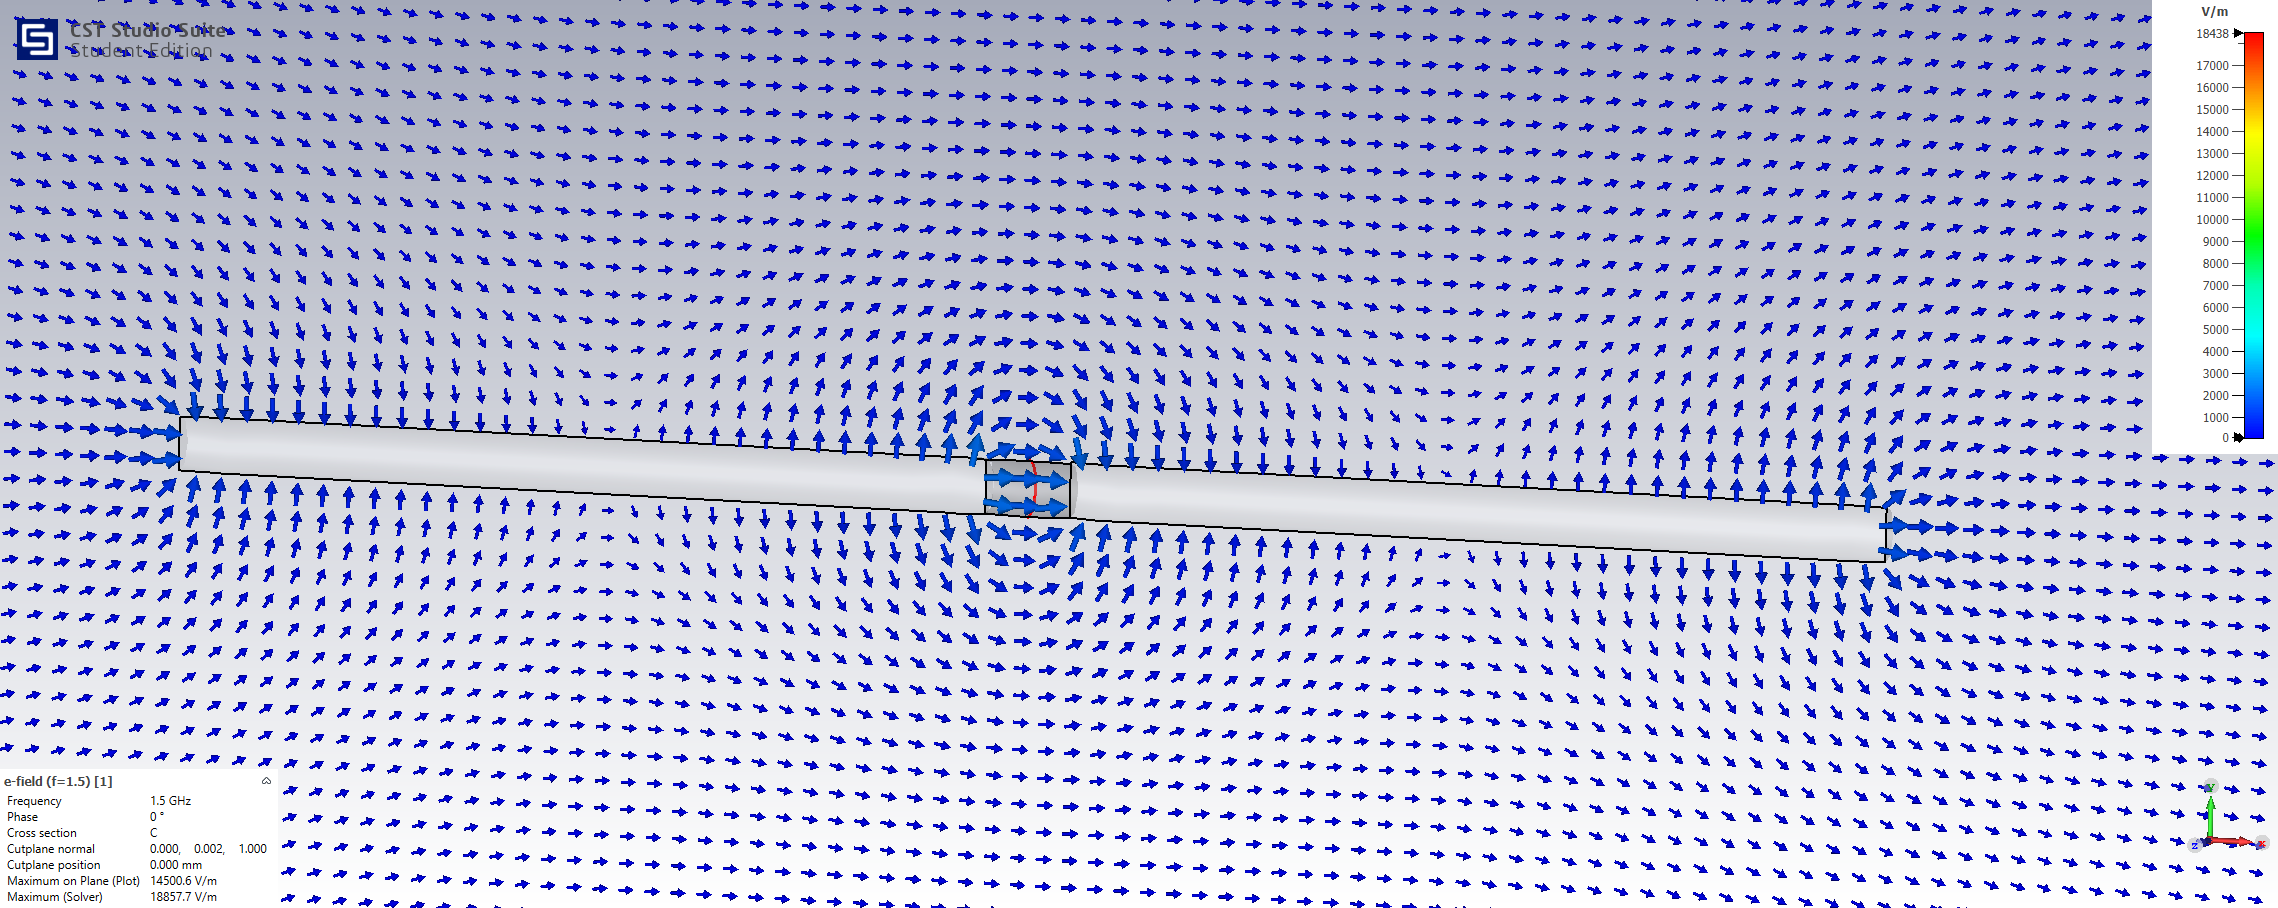
\includegraphics[width=14cm,valign=c]{Images/hw-e-field-xy-plane.png}\hspace{\fill}
	\caption{E-Field as shown from the X-Y plane}  %% Caption for your figure
	\label{fig:hw_e_field_xy}
\end{figure}

The H-Field, shown in Figure \ref{fig:hw_h_field_xy_yz}, shows a similarly expected story. The field curls around the antennas circumference, being most strongest near the port excitation. \linebreak

\begin{figure}[h]
	\centering
	\hspace{\fill}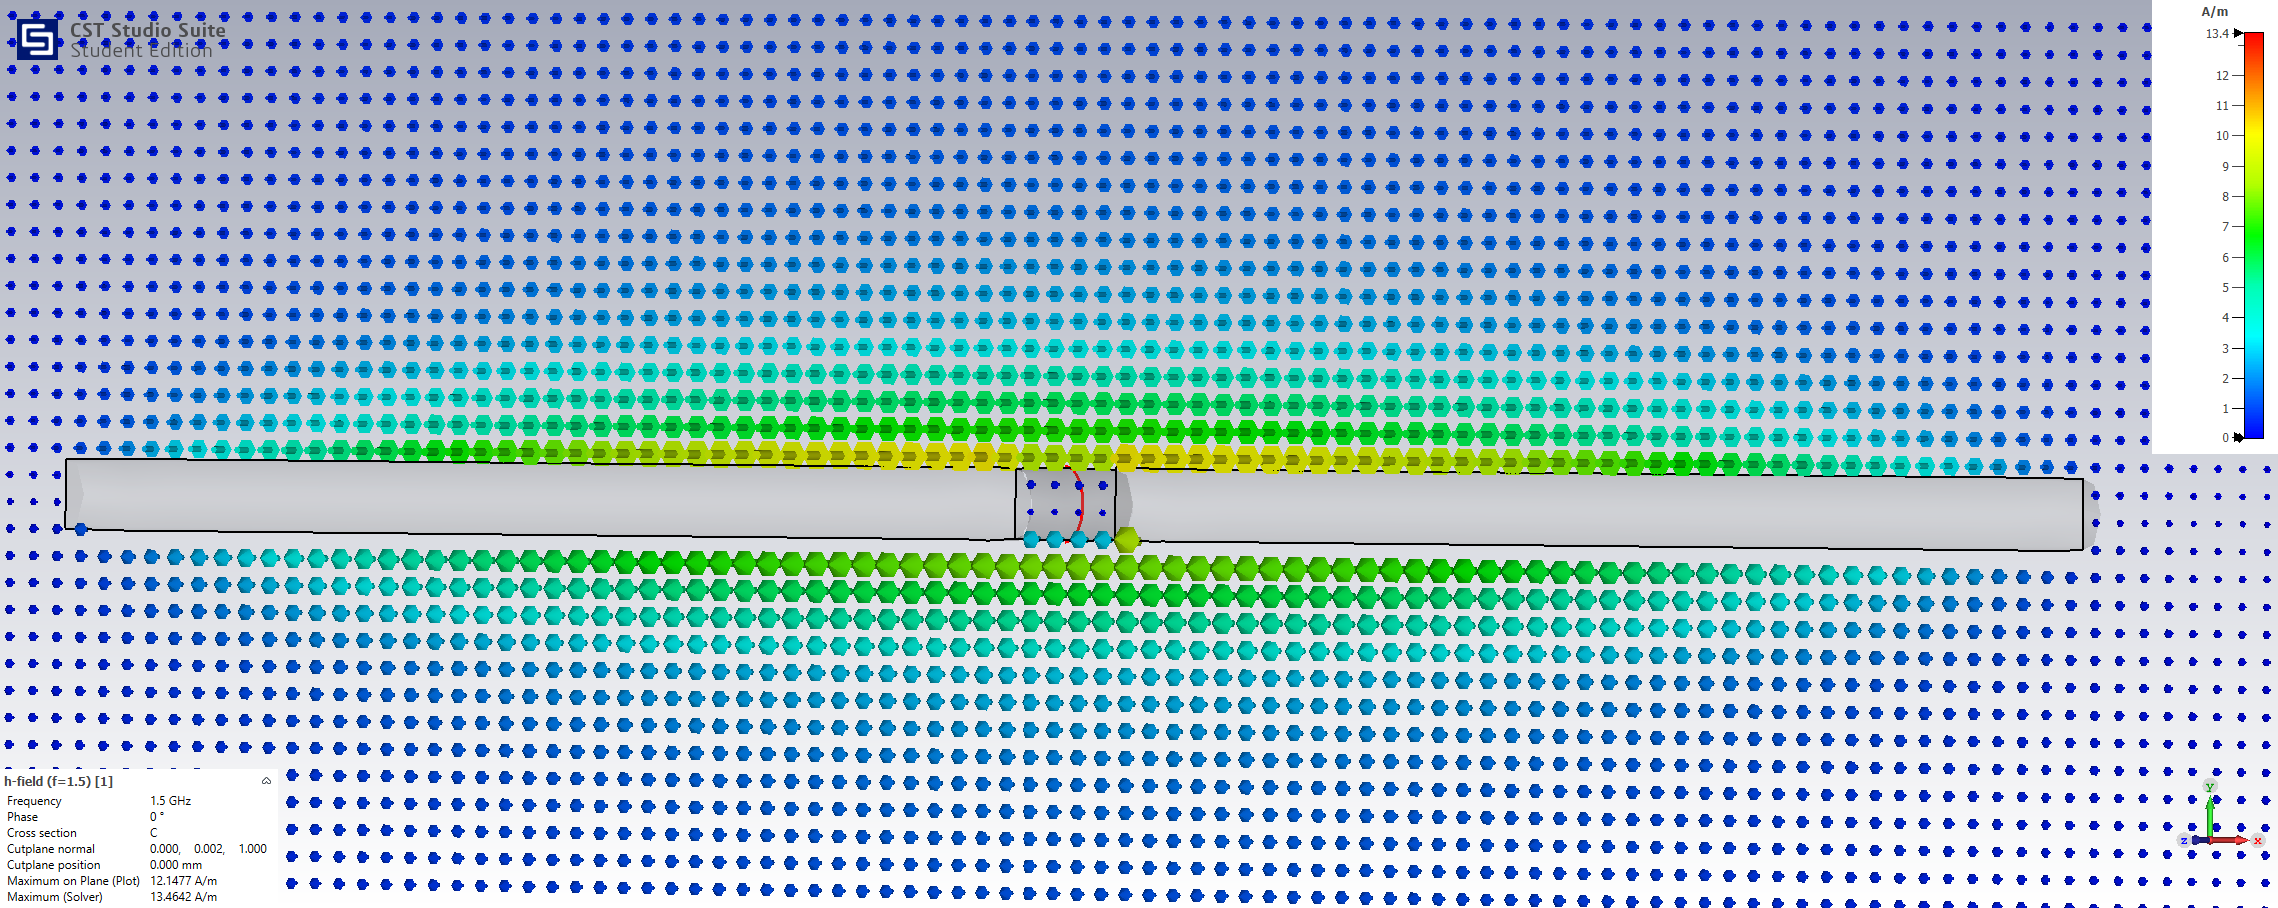
\includegraphics[width=8.5cm,valign=c]{Images/hw-h-field-xy-plane.png}\hspace{\fill}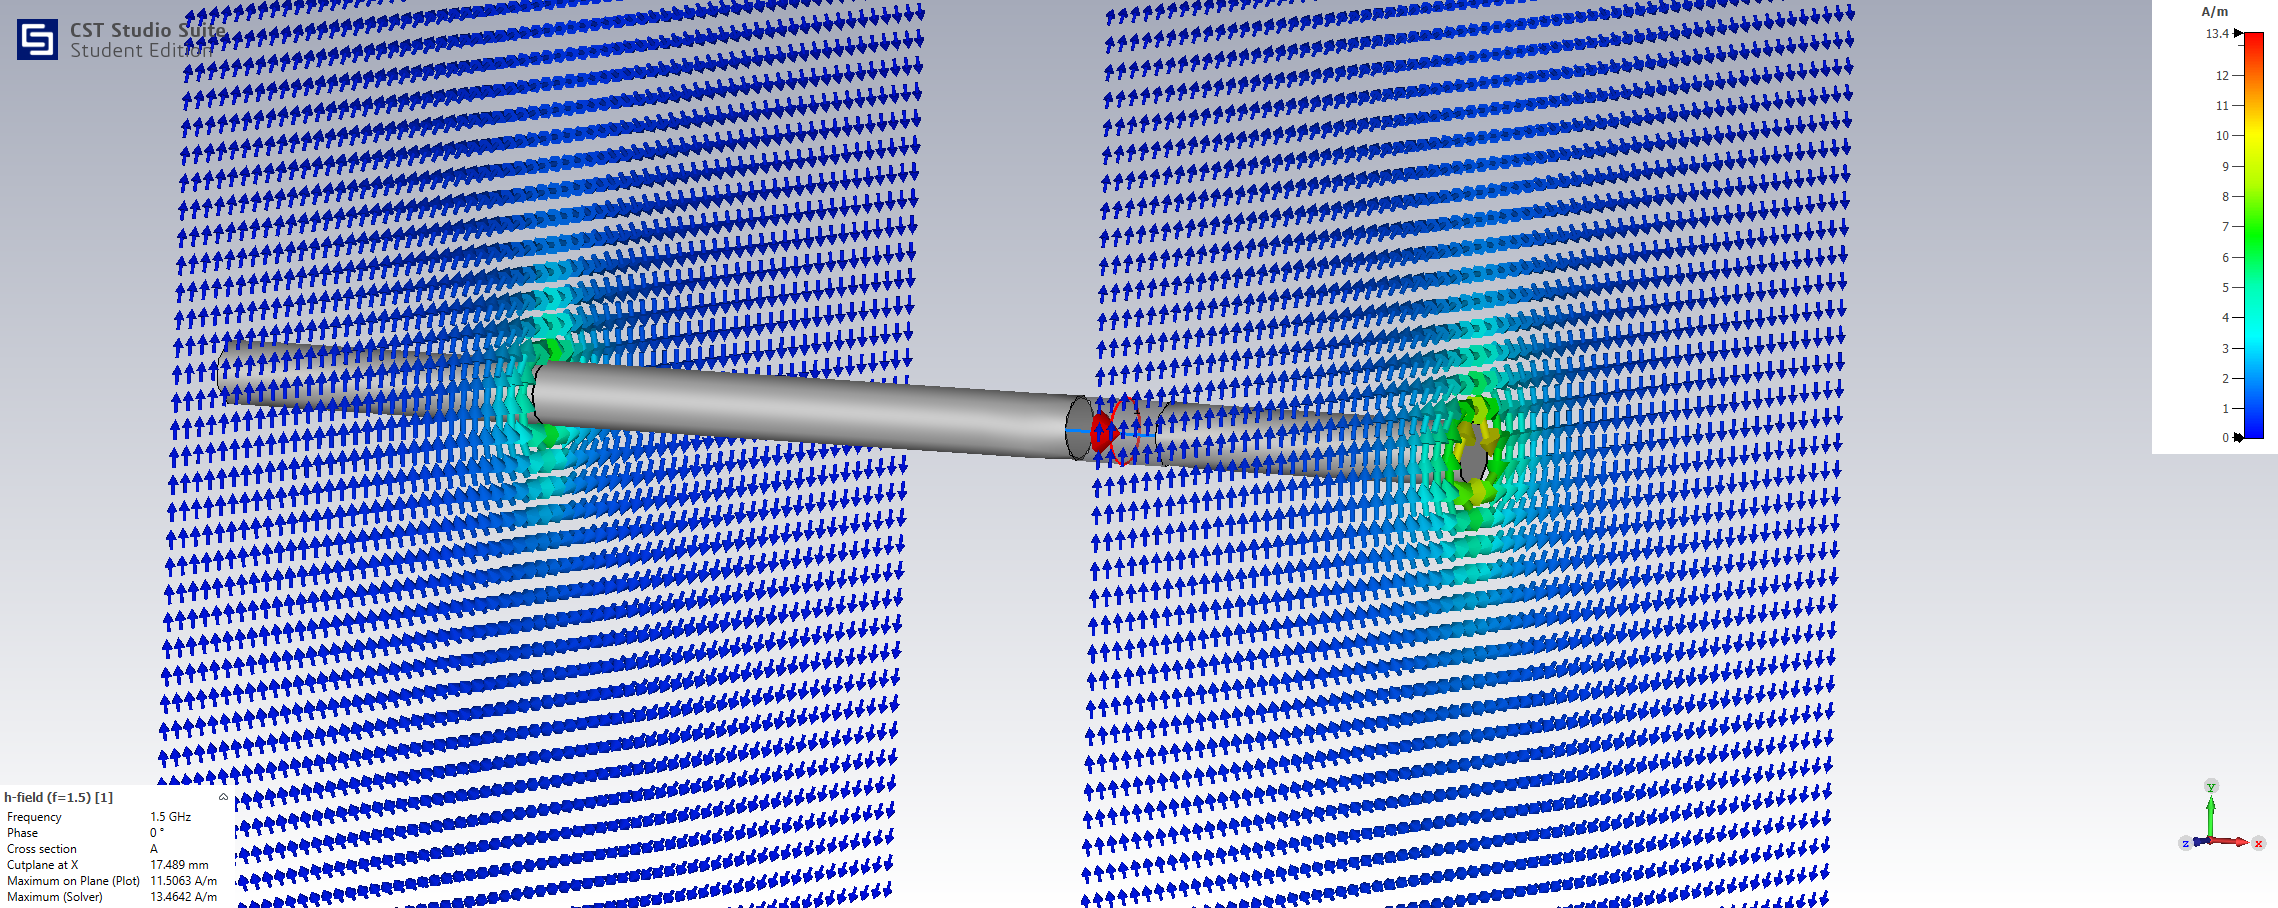
\includegraphics[width=8.5cm,valign=c]{Images/hw-h-field-yz-plane.png}\hspace{\fill}
	\caption{H-Field as shown from the X-Y plane (left) and the Y-Z plane (right)}  %% Caption for your figure
	\label{fig:hw_h_field_xy_yz}
\end{figure}


\newpage




\subsection{Question Three}

The far-field analysis is shown in Figures \ref{fig:hw_ff_3d} and \ref{fig:hw_ff_2d}. The 3D far-field displaying the field attenuation at distance is a ``spherical-torus'' shape. \linebreak

\begin{figure}[h]
	\centering
	\hspace{\fill}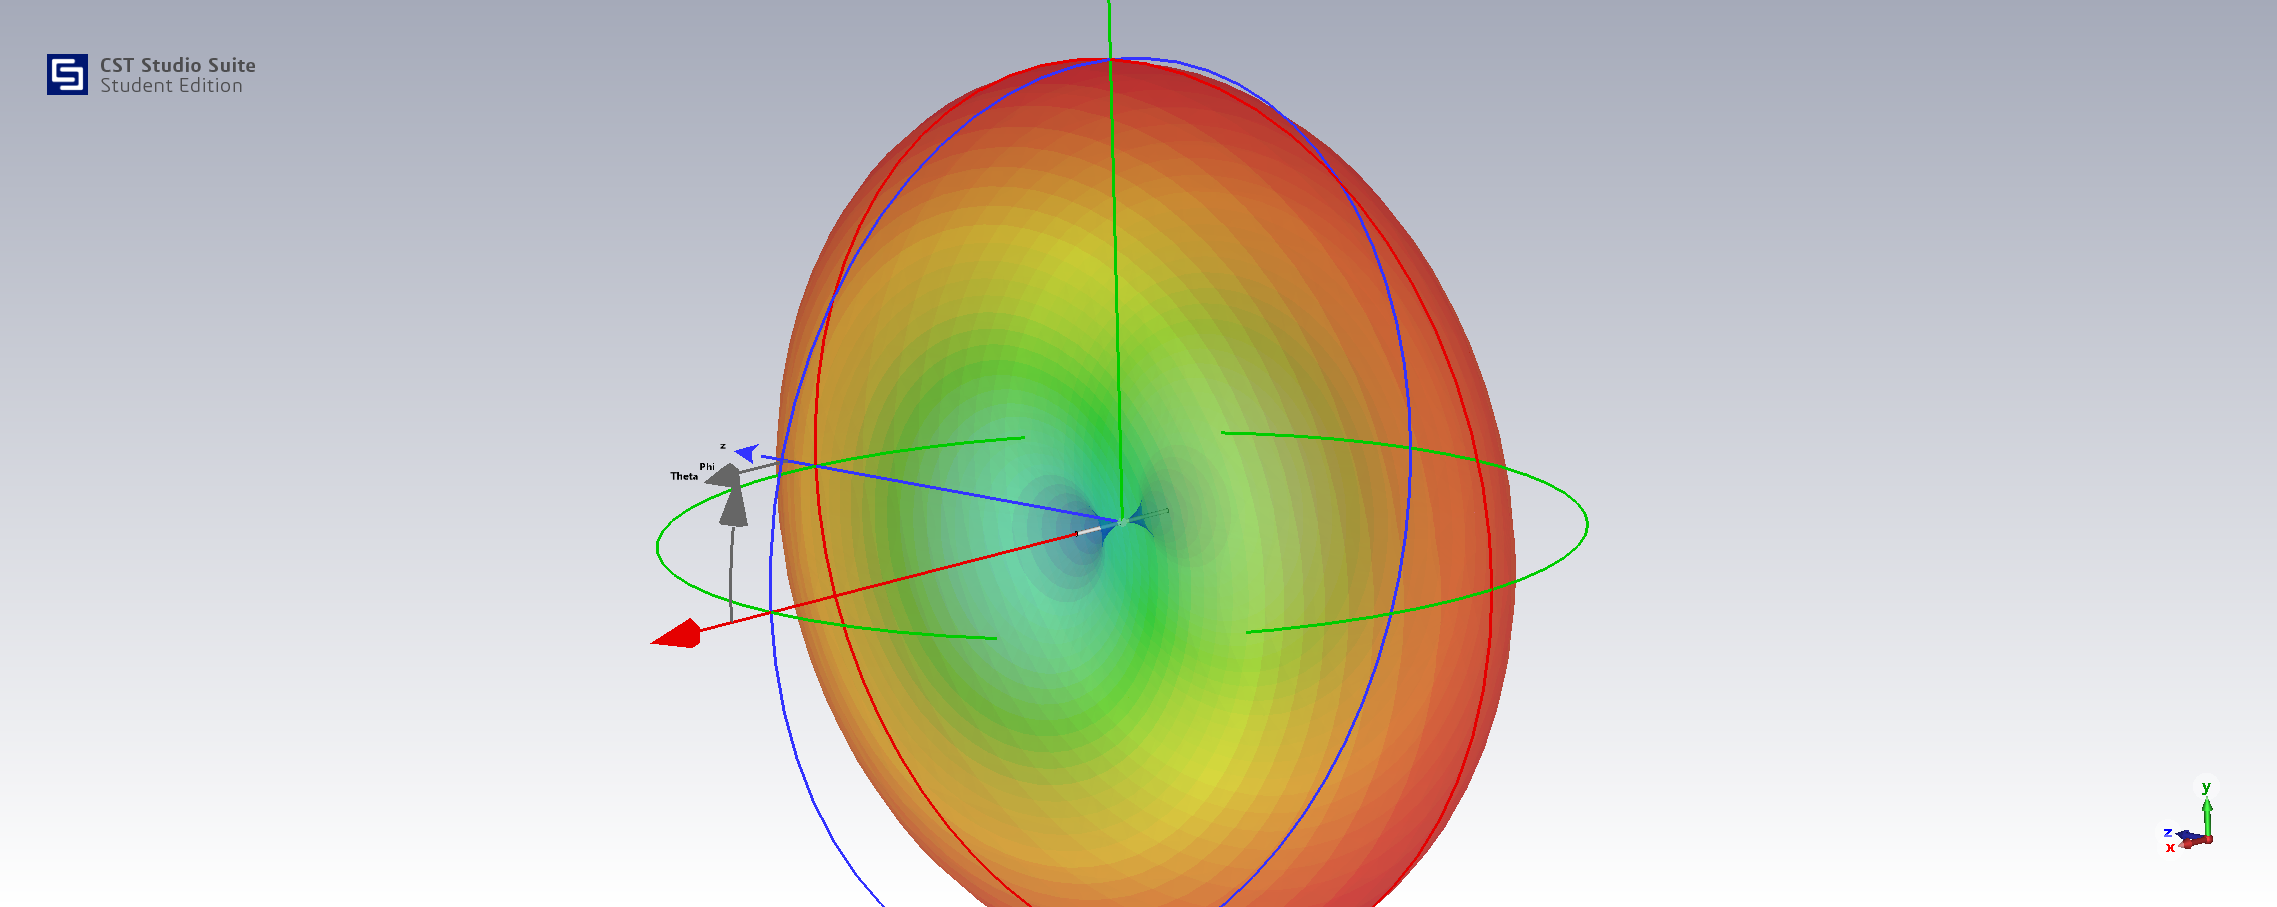
\includegraphics[width=14cm,valign=c]{Images/hw-farfield-plot-3d.png}\hspace{\fill}
	\caption{the 3D far-field analysis showing the ``spherical torus'' radiation pattern}  %% Caption for your figure
	\label{fig:hw_ff_3d}
\end{figure}

The X-Y view shows that the antenna is highly attenuated in the X plane compared to the Y and Z planes, where it is significantly stronger. \linebreak

\begin{figure}[h]
	\centering
	\hspace{\fill}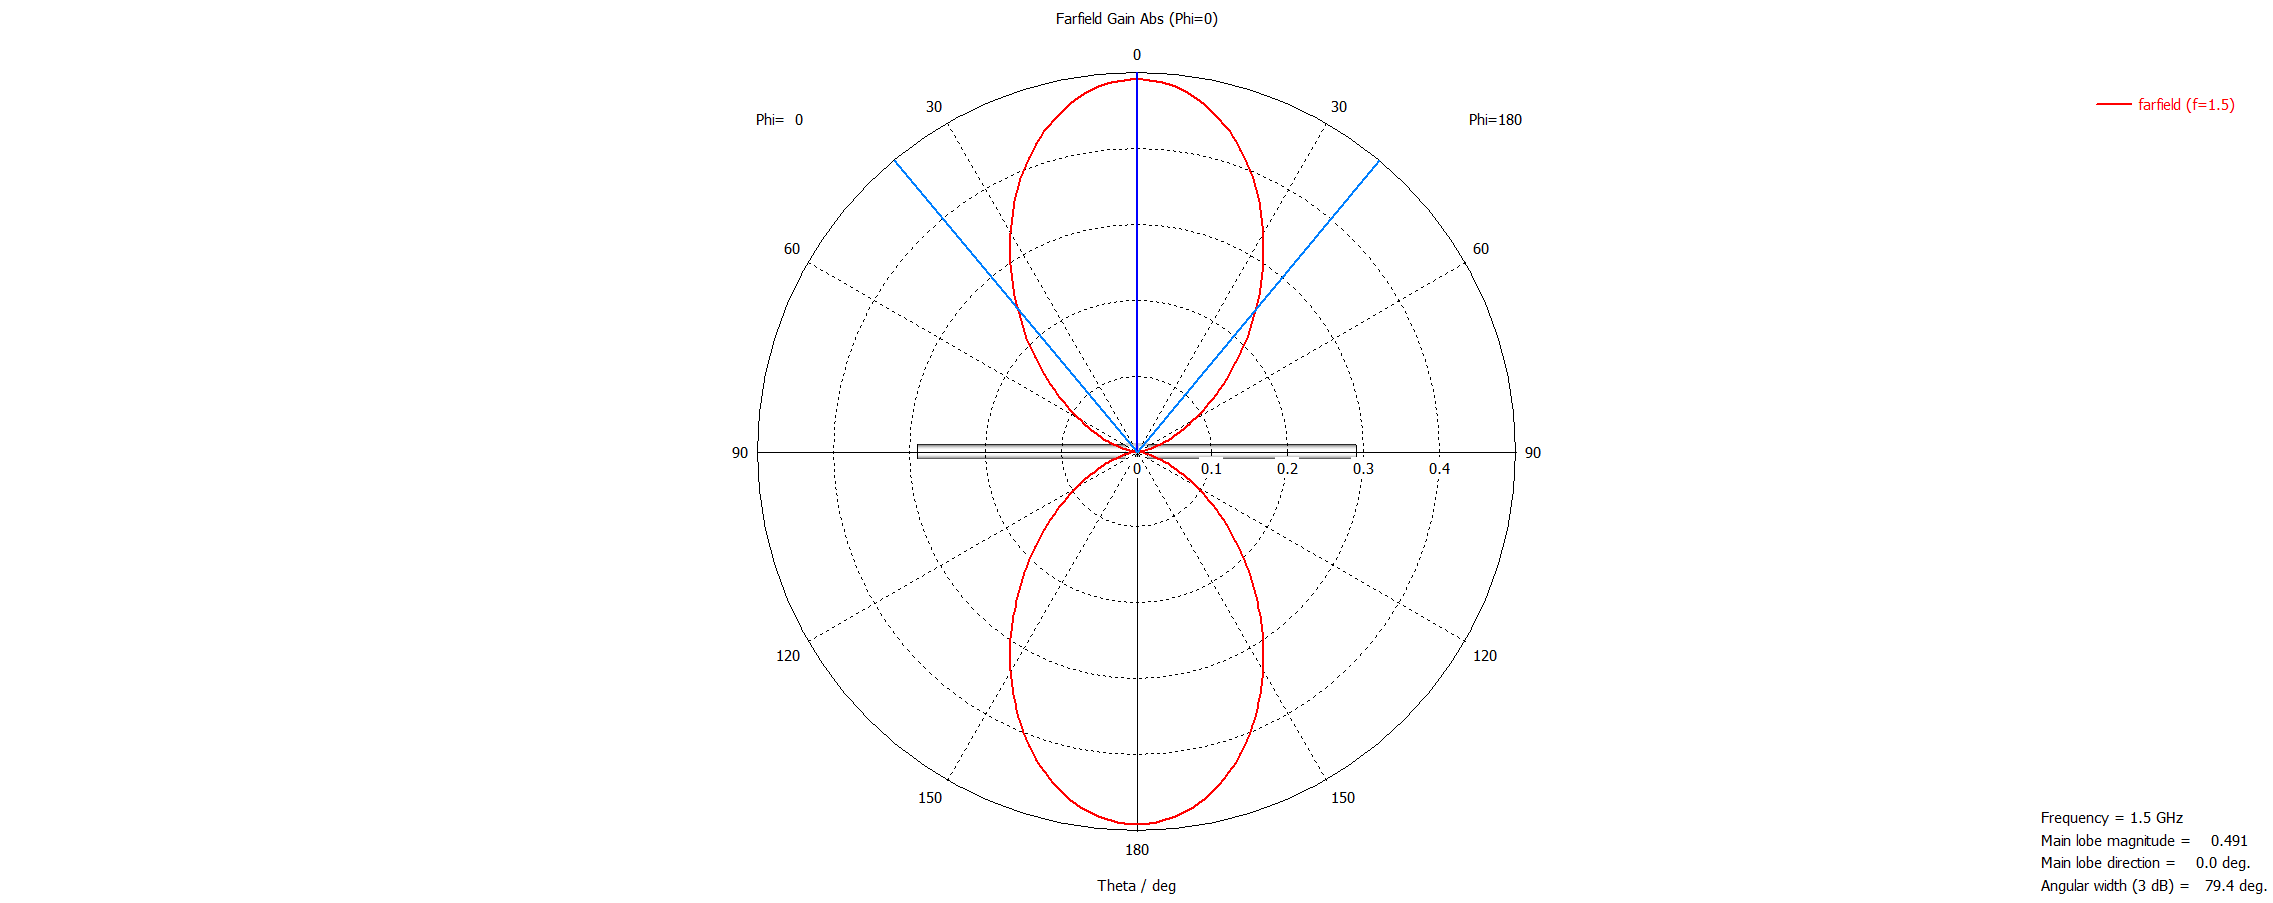
\includegraphics[width=9cm,valign=c]{Images/hw-farfield-plot-xy-plane.png}\hspace{\fill}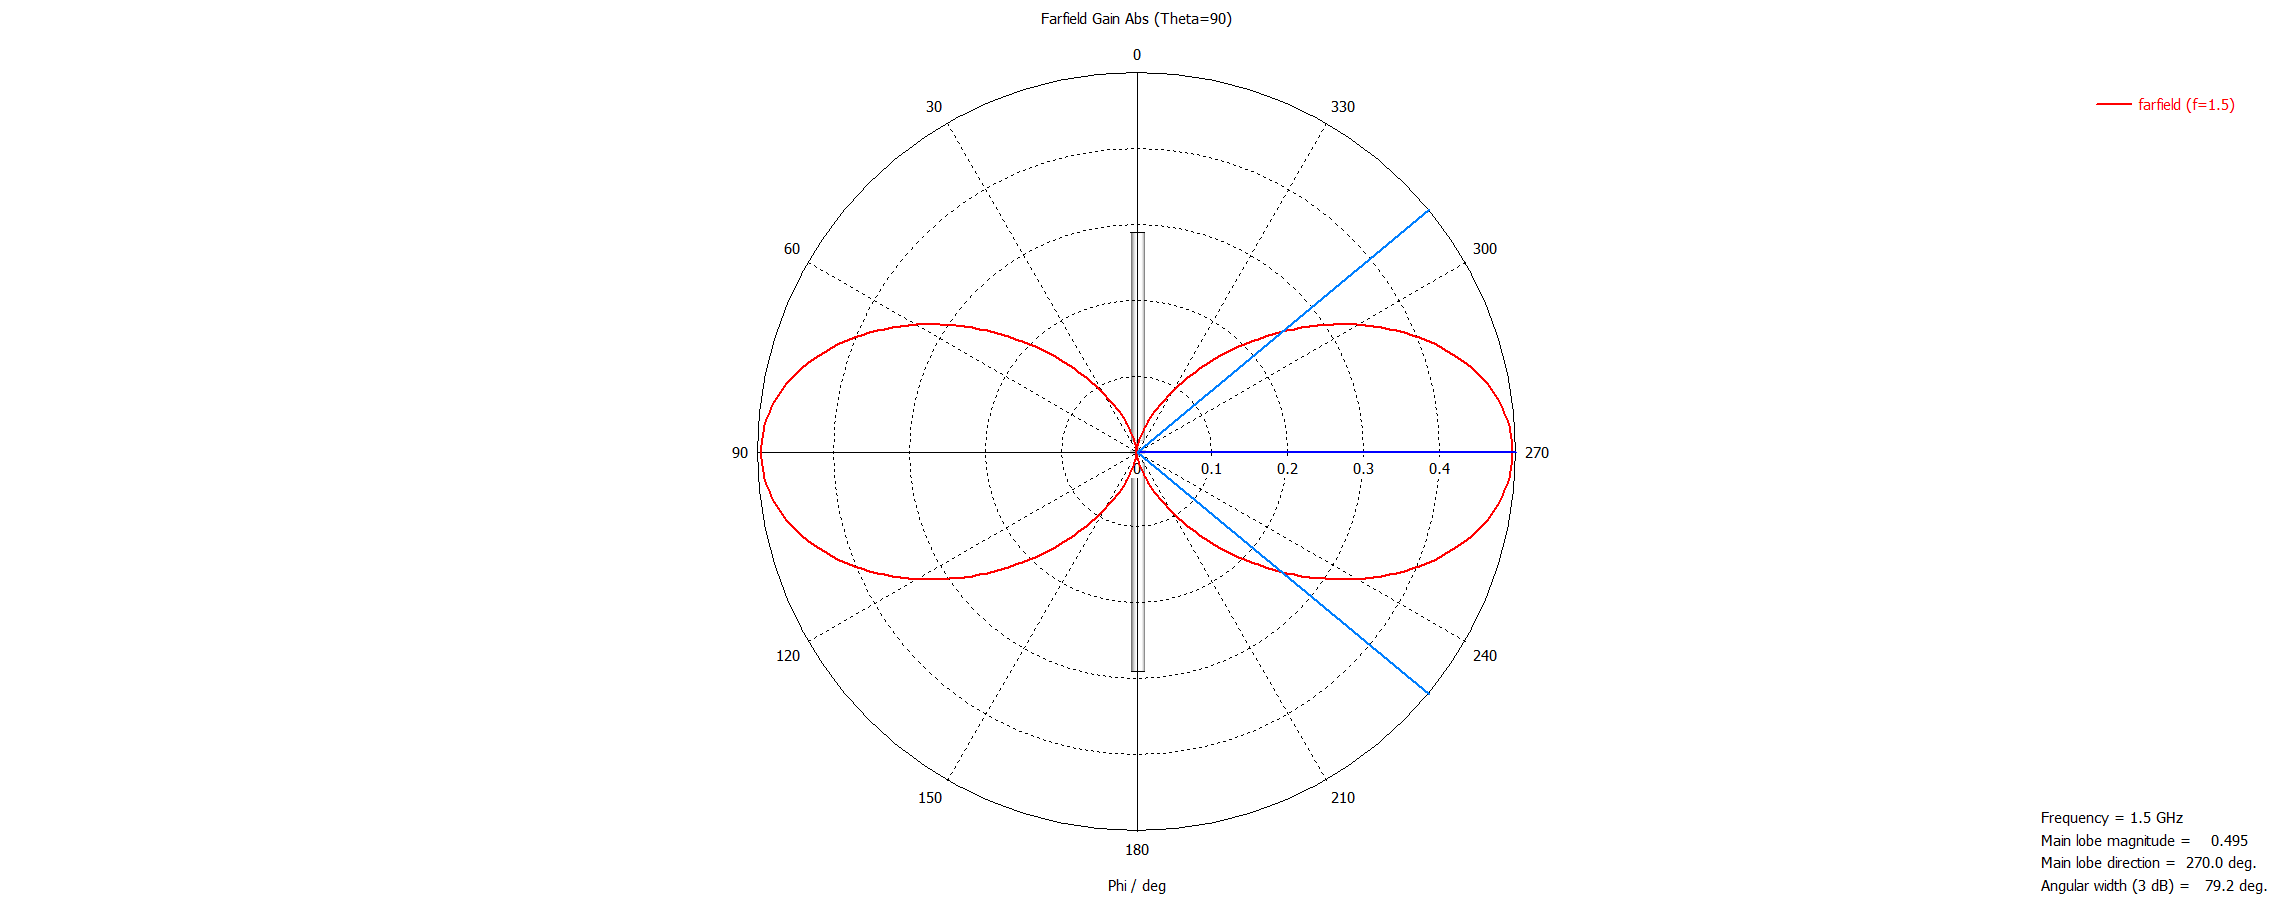
\includegraphics[width=9cm,valign=c]{Images/hw-farfield-plot-xz-plane.png}\hspace{\fill}
	\caption{Far-Field in 2D shown from the X-Y plane (left) and the X-Z plane (right)}  %% Caption for your figure
	\label{fig:hw_ff_2d}
\end{figure}

\newpage



\section{Quarter-Wavelength Monopole Antenna}
\subsection{Question Four}

Repeating the steps I carried out in the first question, I designed and simulated the results for the monopole antenna, the final S(1,1) parameters, dimensions, and real/complex impedance values are shown below in Figures \ref{fig:qw_s11_params_init_sweeps}, \ref{fig:qw_s11_dimesions_final}, and \ref{fig:qw_impedance}.

\begin{figure}[h]
	\centering
	\hspace{\fill}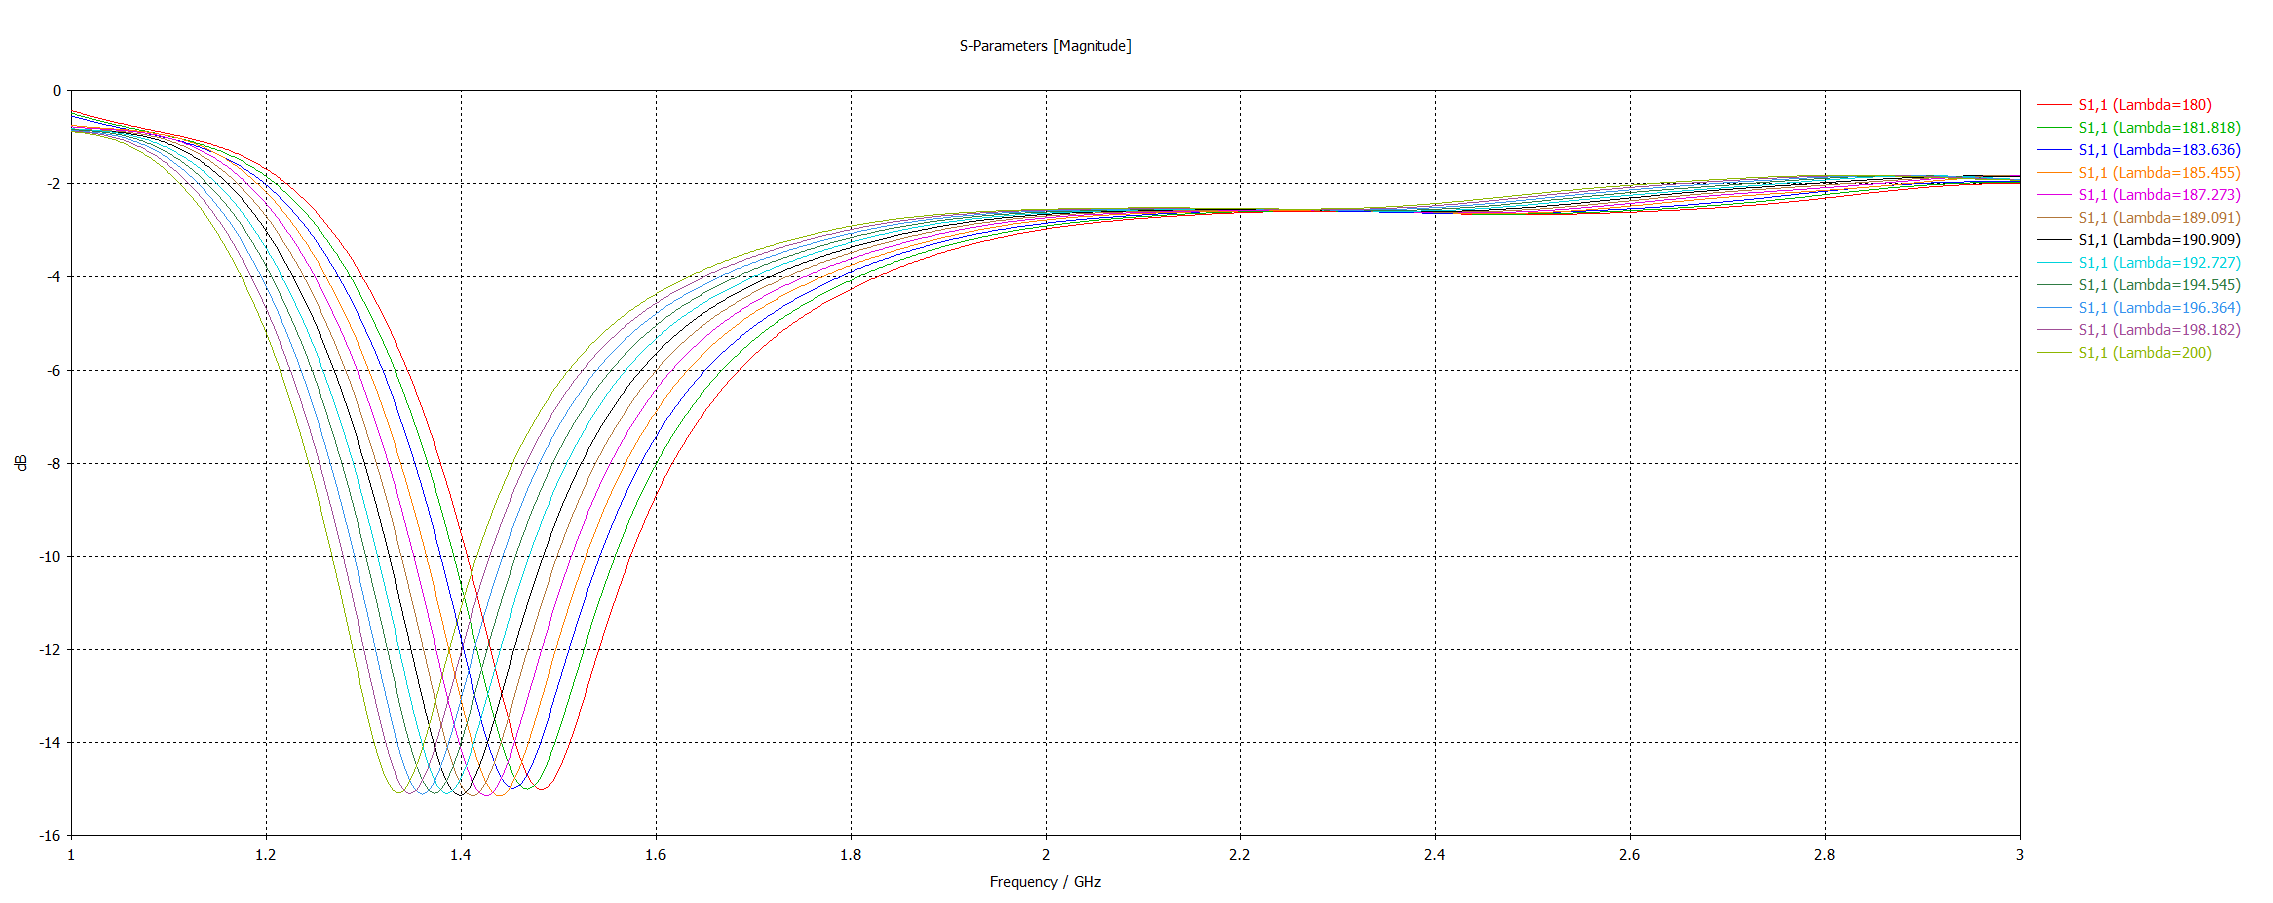
\includegraphics[width=9cm,valign=c]{Images/qw-lambda-sweep-broad-S1,1.png}\hspace{\fill}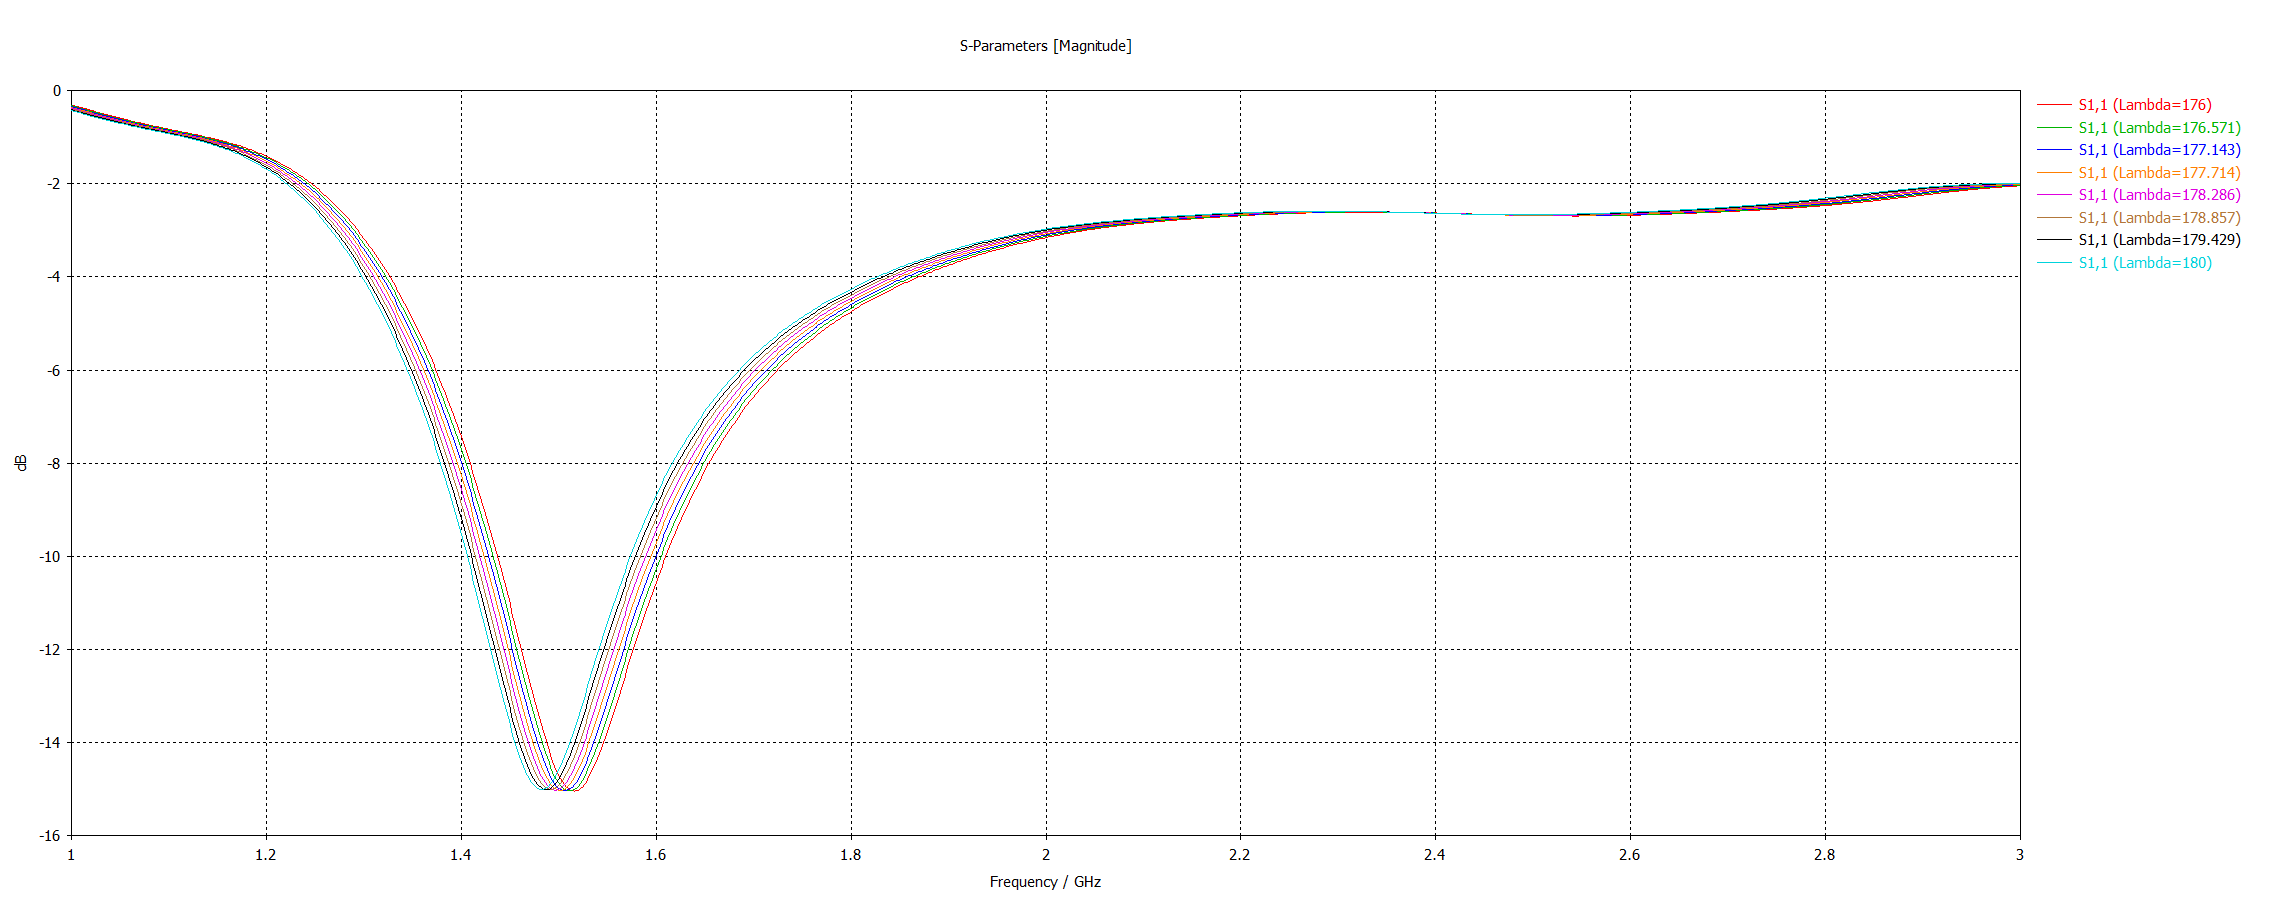
\includegraphics[width=9cm,valign=c]{Images/qw-lambda-sweep-narrow-S1,1.png}\hspace{\fill}
	\caption{The monopole's S1,1 Parameters for initially calculated wavelength (bottom) and the broad and narrow parameter sweeps (top left and right respectively)}  %% Caption for your figure
	\label{fig:qw_s11_params_init_sweeps}
\end{figure}

\begin{figure}[h!]
	\centering
	\hspace{\fill}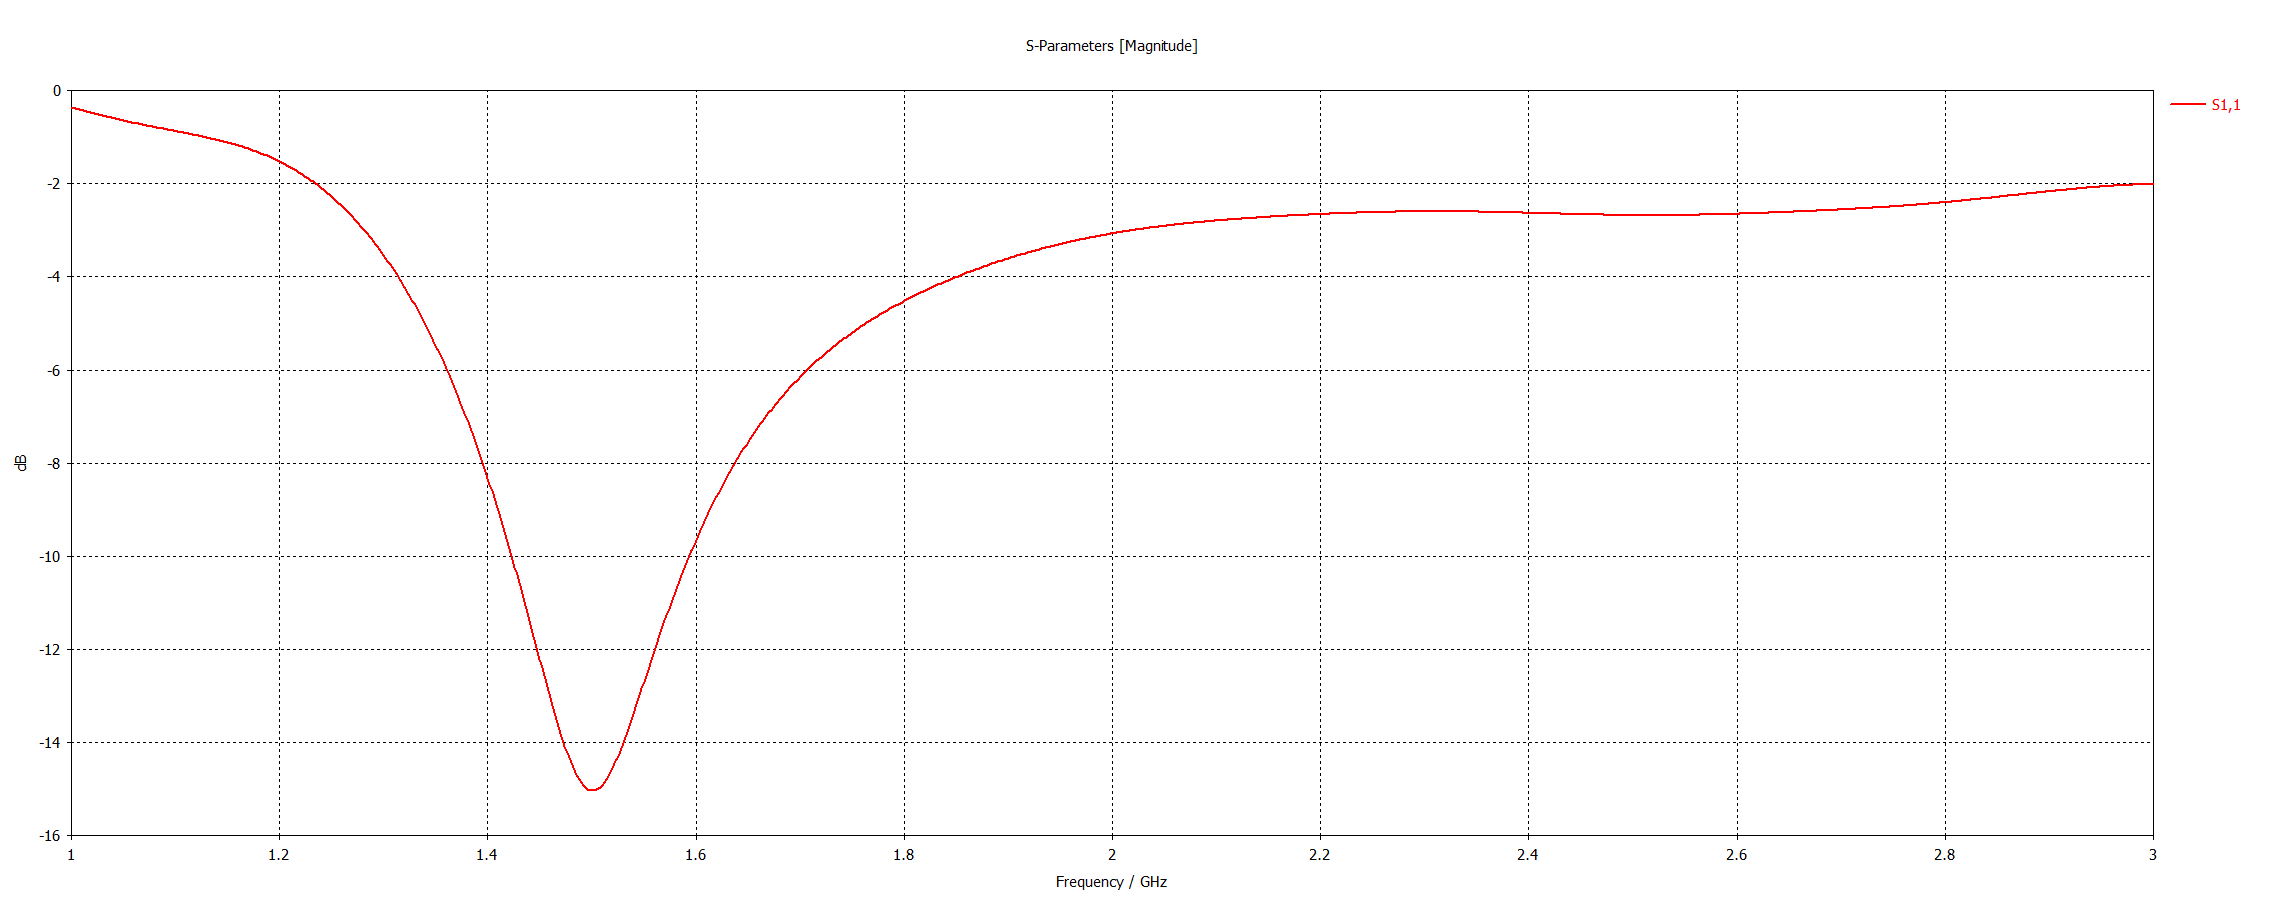
\includegraphics[width=10cm,valign=c]{Images/qw-lambda-177.8-S1,1.png}\hspace{\fill}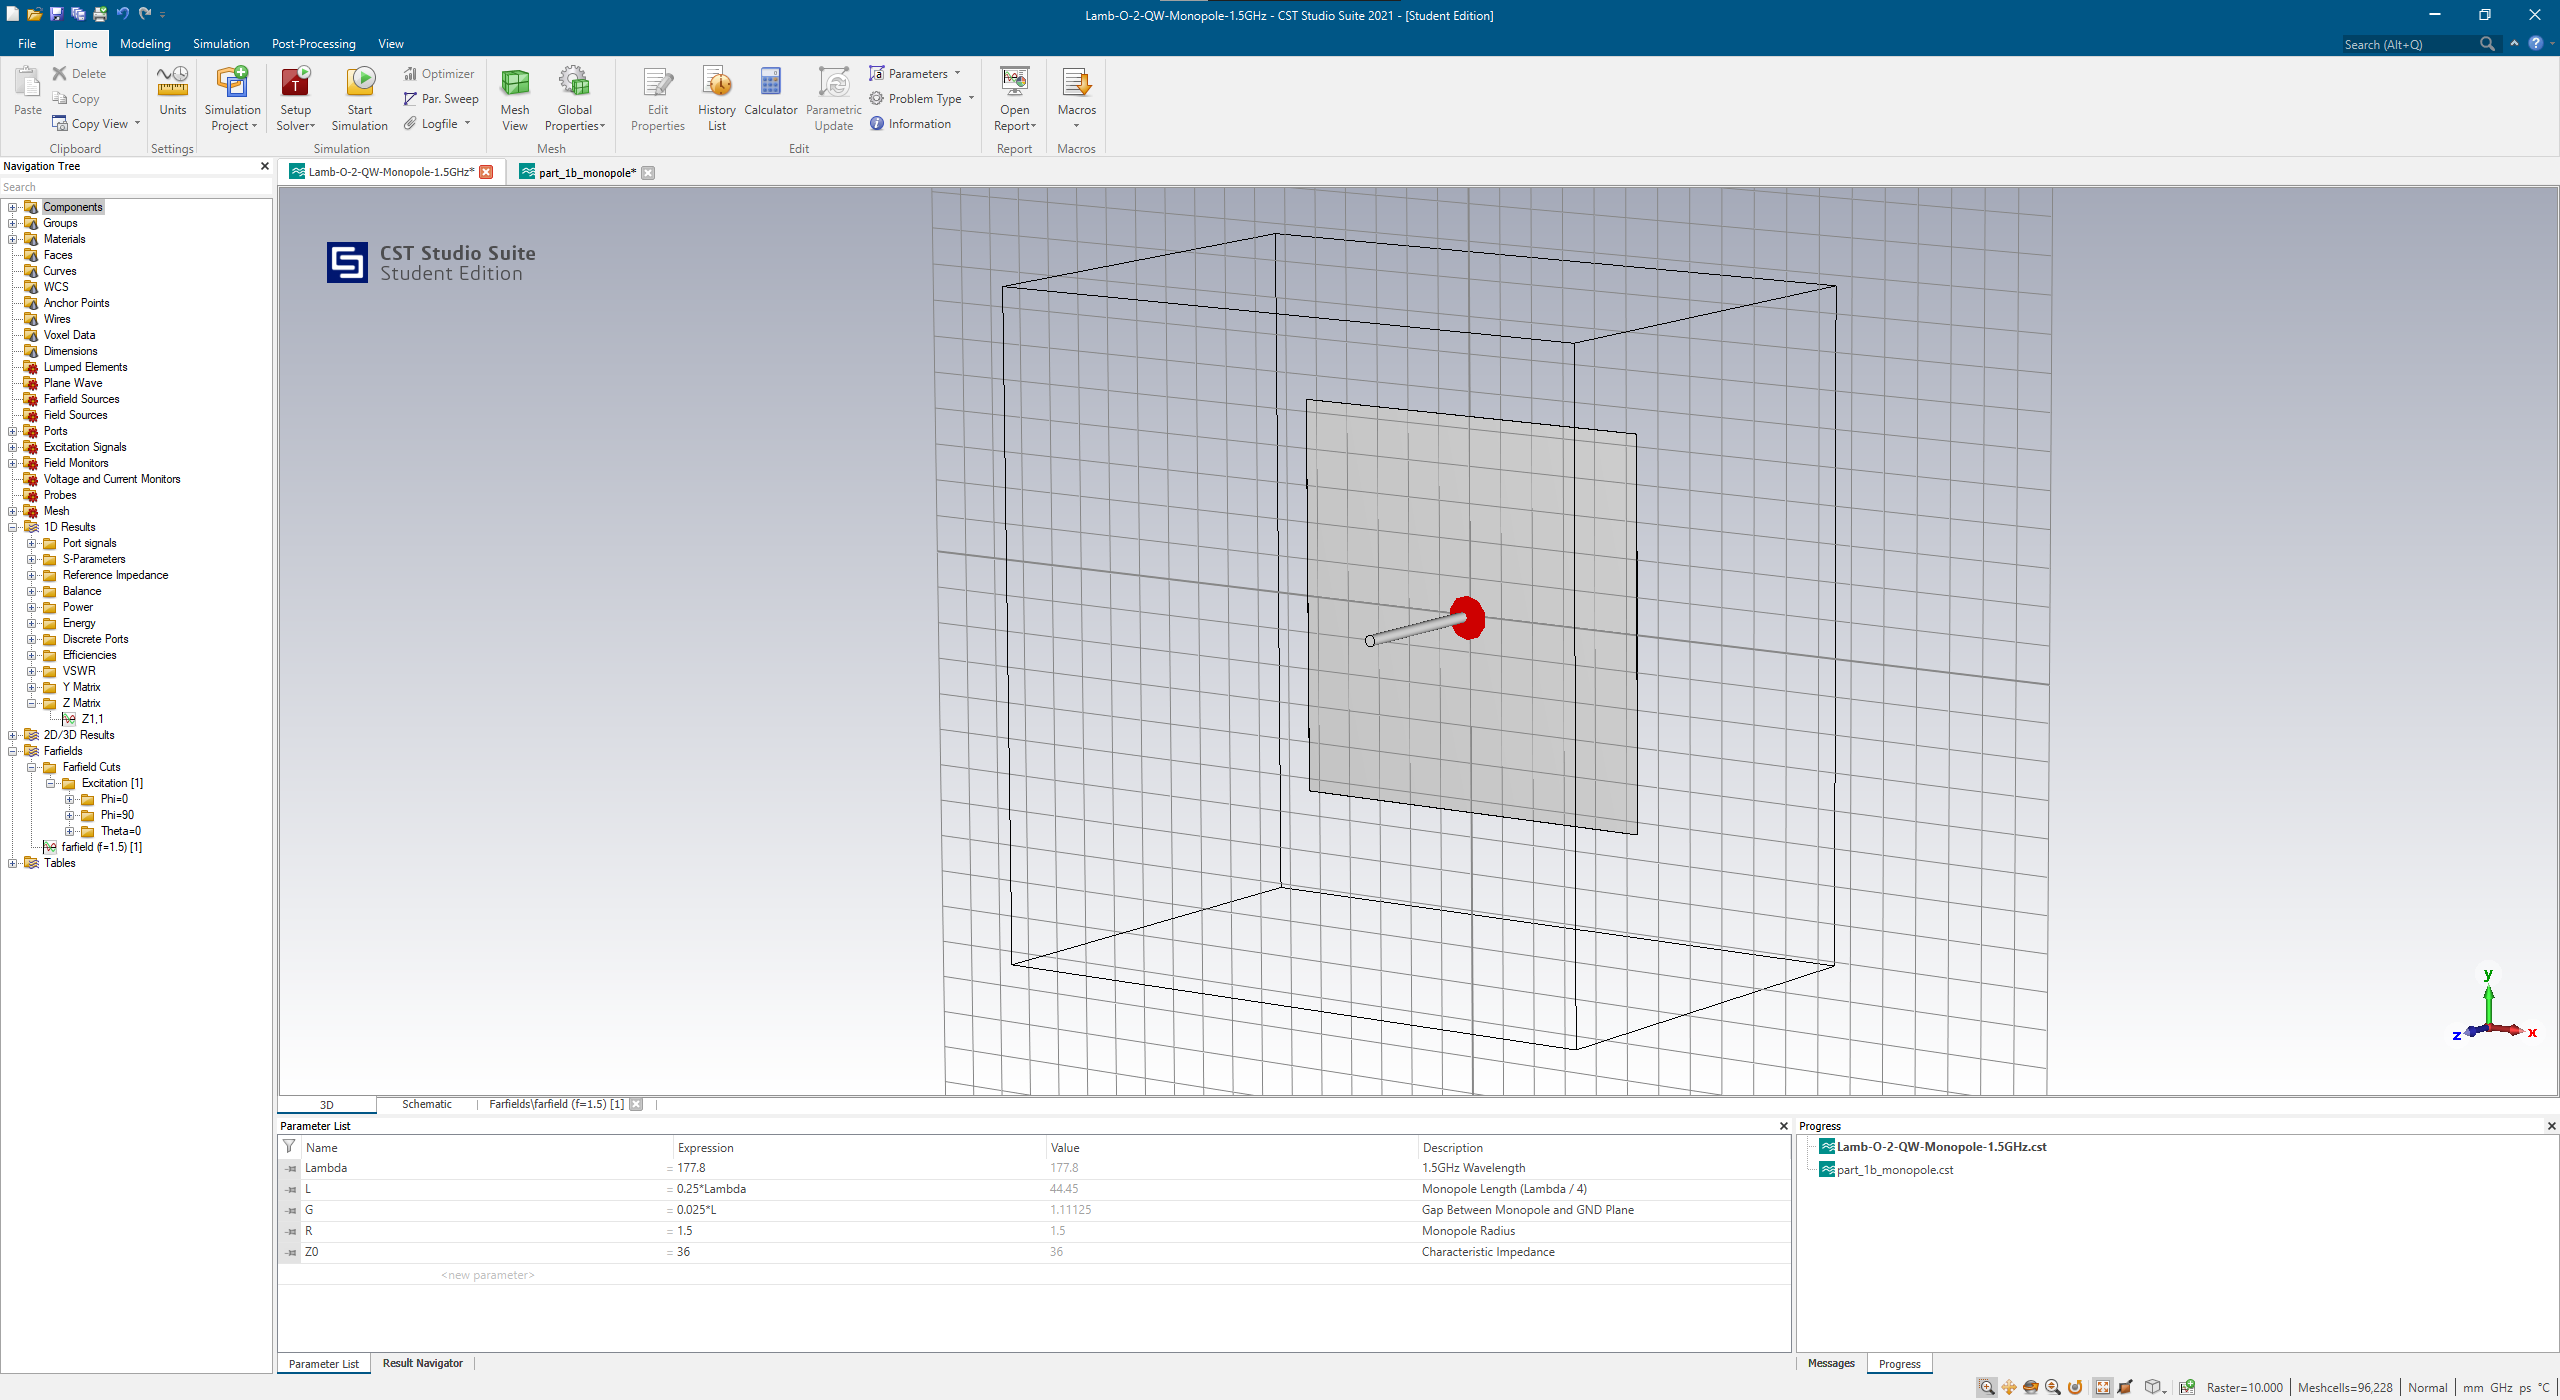
\includegraphics[width=8cm,valign=c]{Images/qw-final-dimens.png}\hspace{\fill}
	\caption{The final S(1,1) parameters (left) and the final dimensions and design of the monopole (right)}
	\label{fig:qw_s11_dimesions_final}
\end{figure}

\begin{figure}[h]
	\centering
	\hspace{\fill}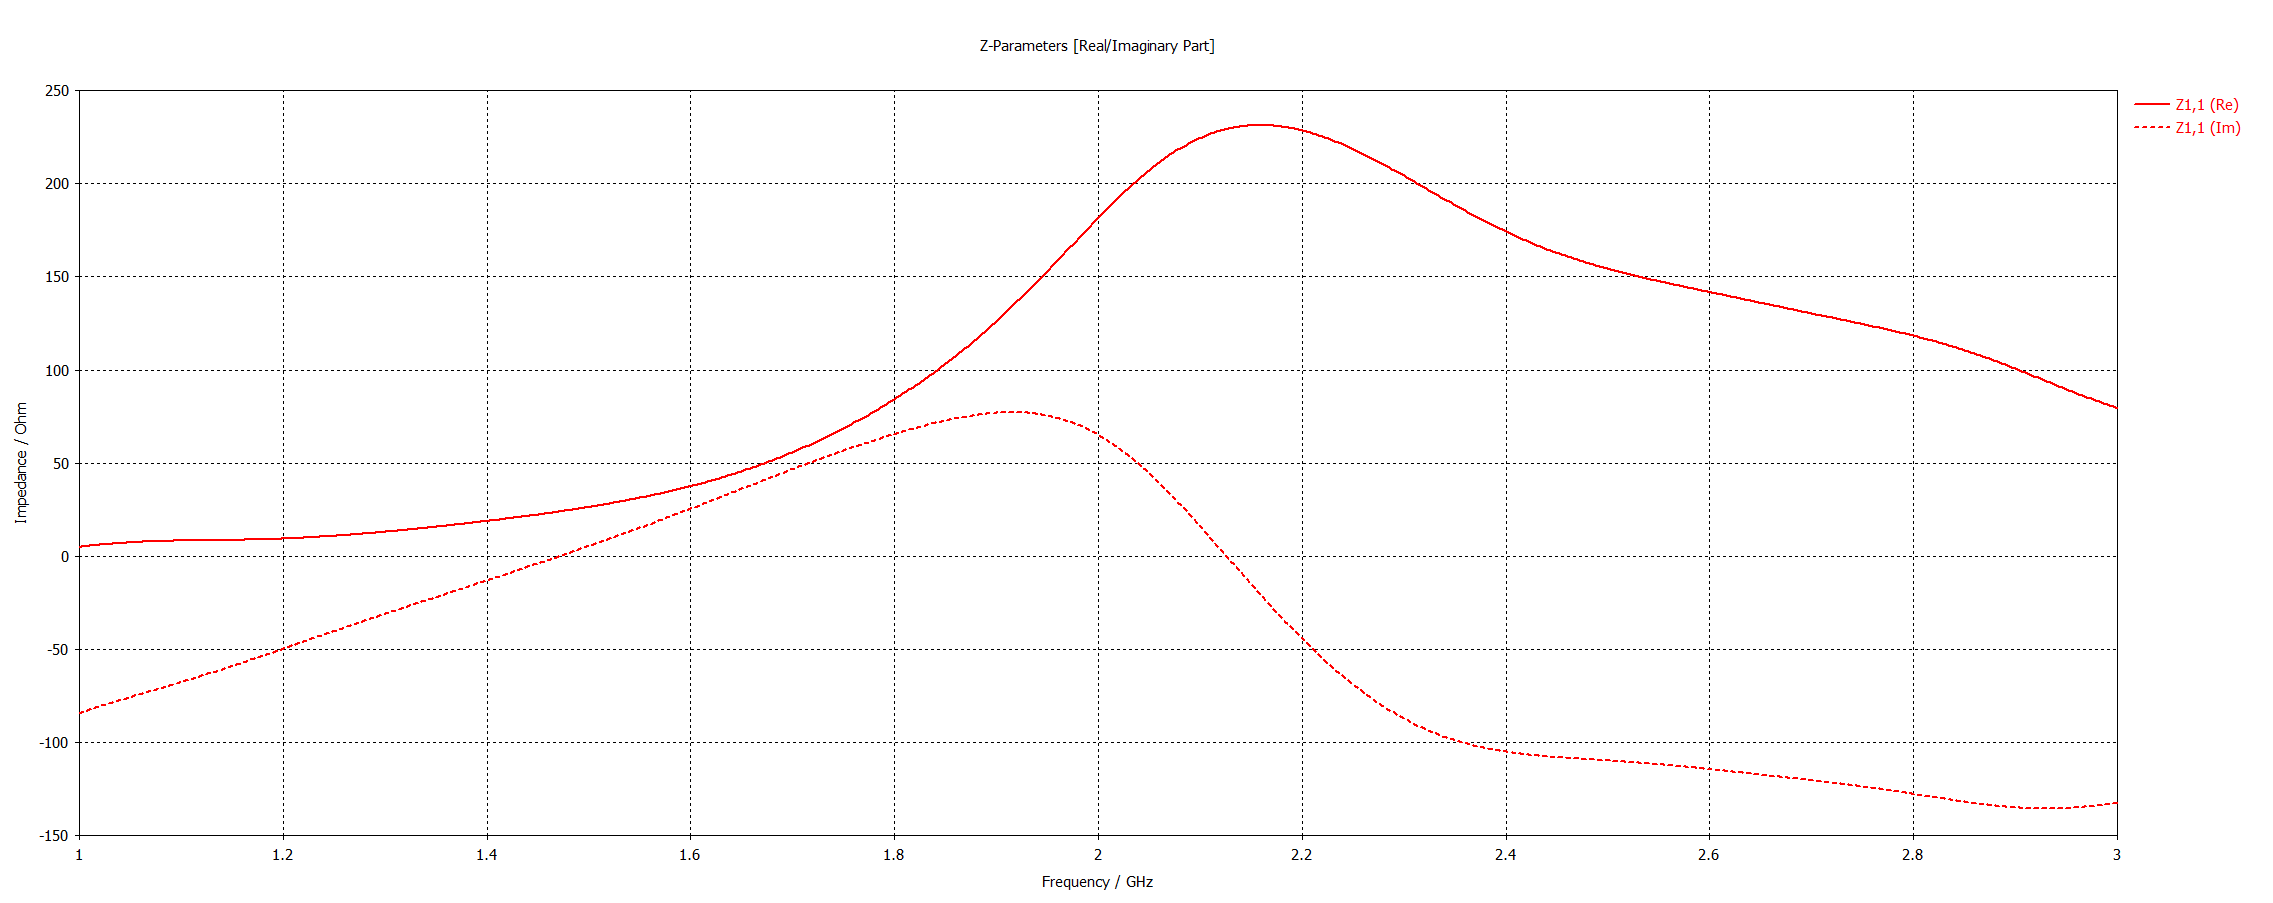
\includegraphics[width=14cm,valign=c]{Images/qw-real-imag-impedance.png}\hspace{\fill}
	\caption{The impedance graph across frequency for the monopole antenna}  %% Caption for your figure
	\label{fig:qw_impedance}
\end{figure}

\newpage




\subsection{Question Five}

The far-field analysis of the monopole antenna is shown in Figures \ref{fig:qw_ff_3d} and \ref{fig:qw_ff_2d}. One can see that it's field is far more limited than that of the dipole. \linebreak

\begin{figure}[h]
	\centering
	\hspace{\fill}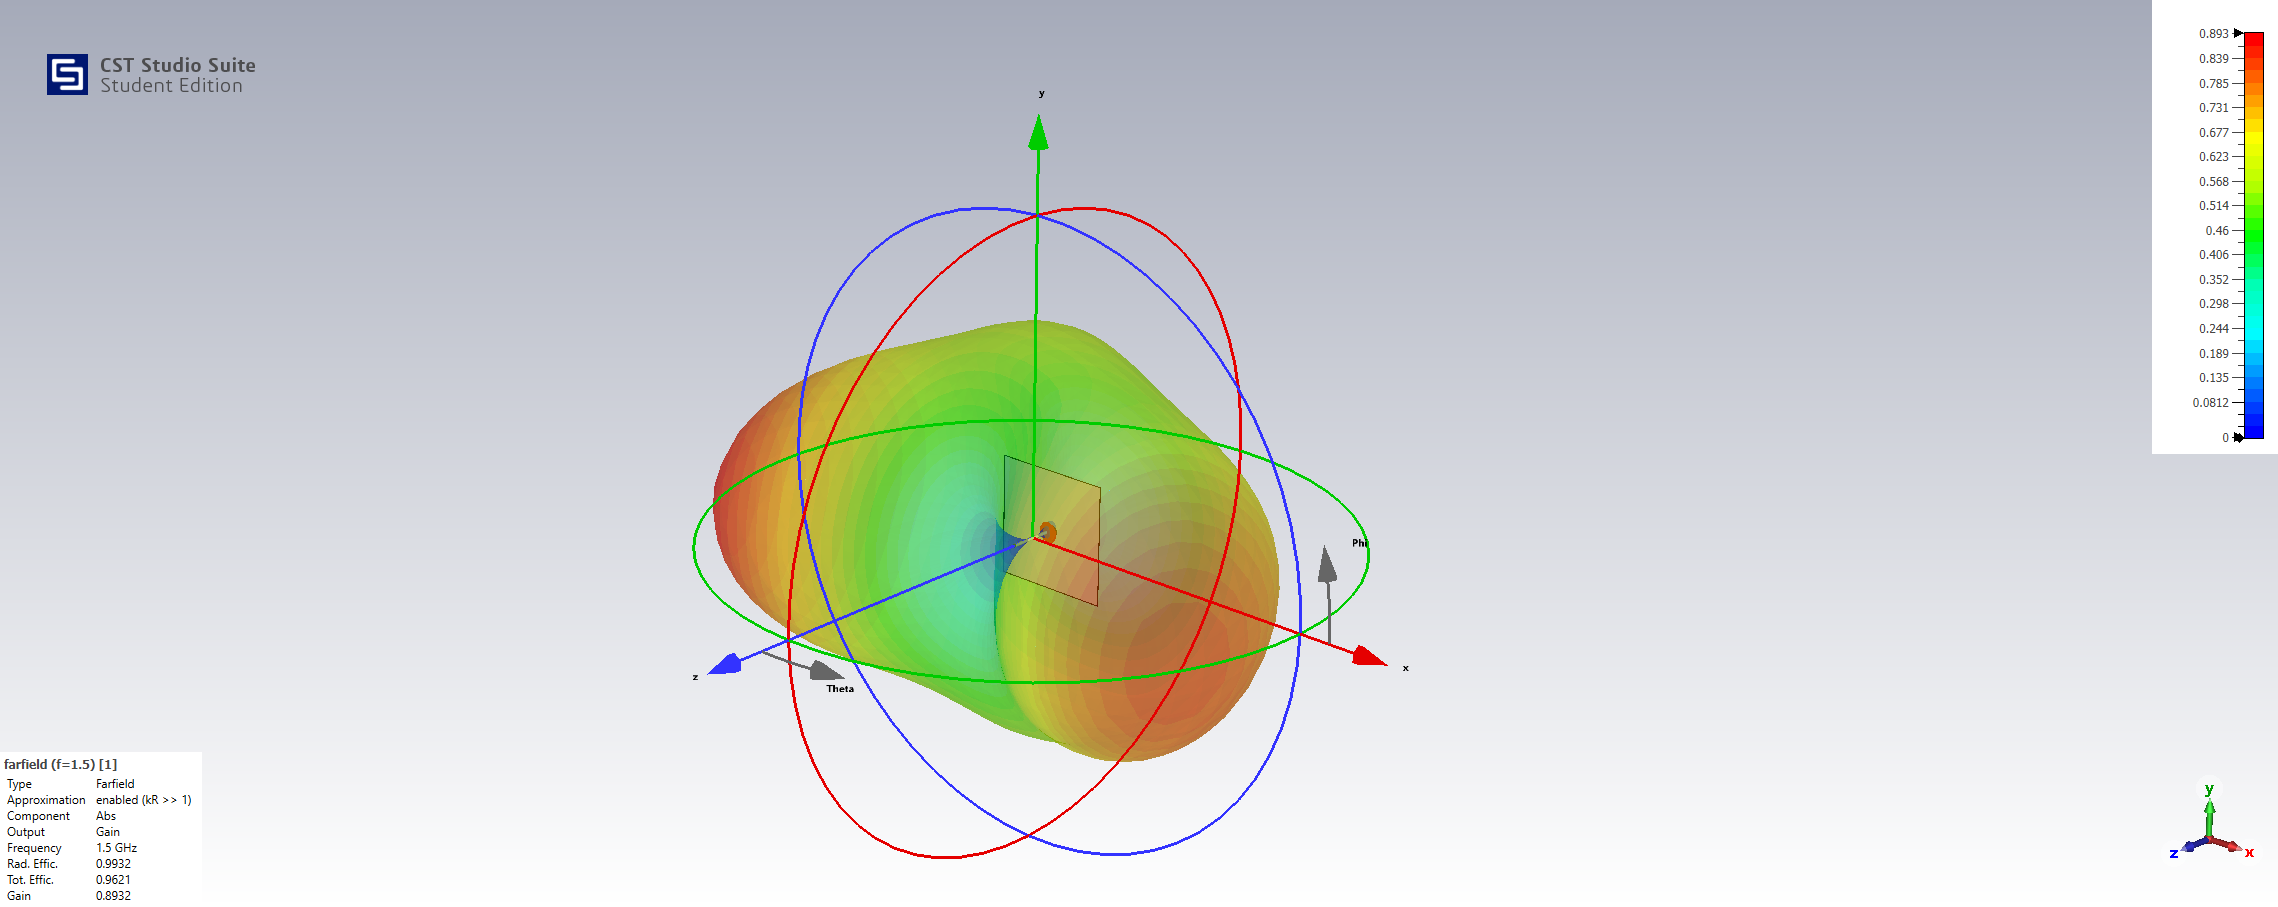
\includegraphics[width=14cm,valign=c]{Images/qw-farfield-plot-3d.png}\hspace{\fill}
	\caption{The 3D far-field analysis showing the radiation pattern of the monopole}  %% Caption for your figure
	\label{fig:qw_ff_3d}
\end{figure}

\begin{figure}[h]
	\centering
	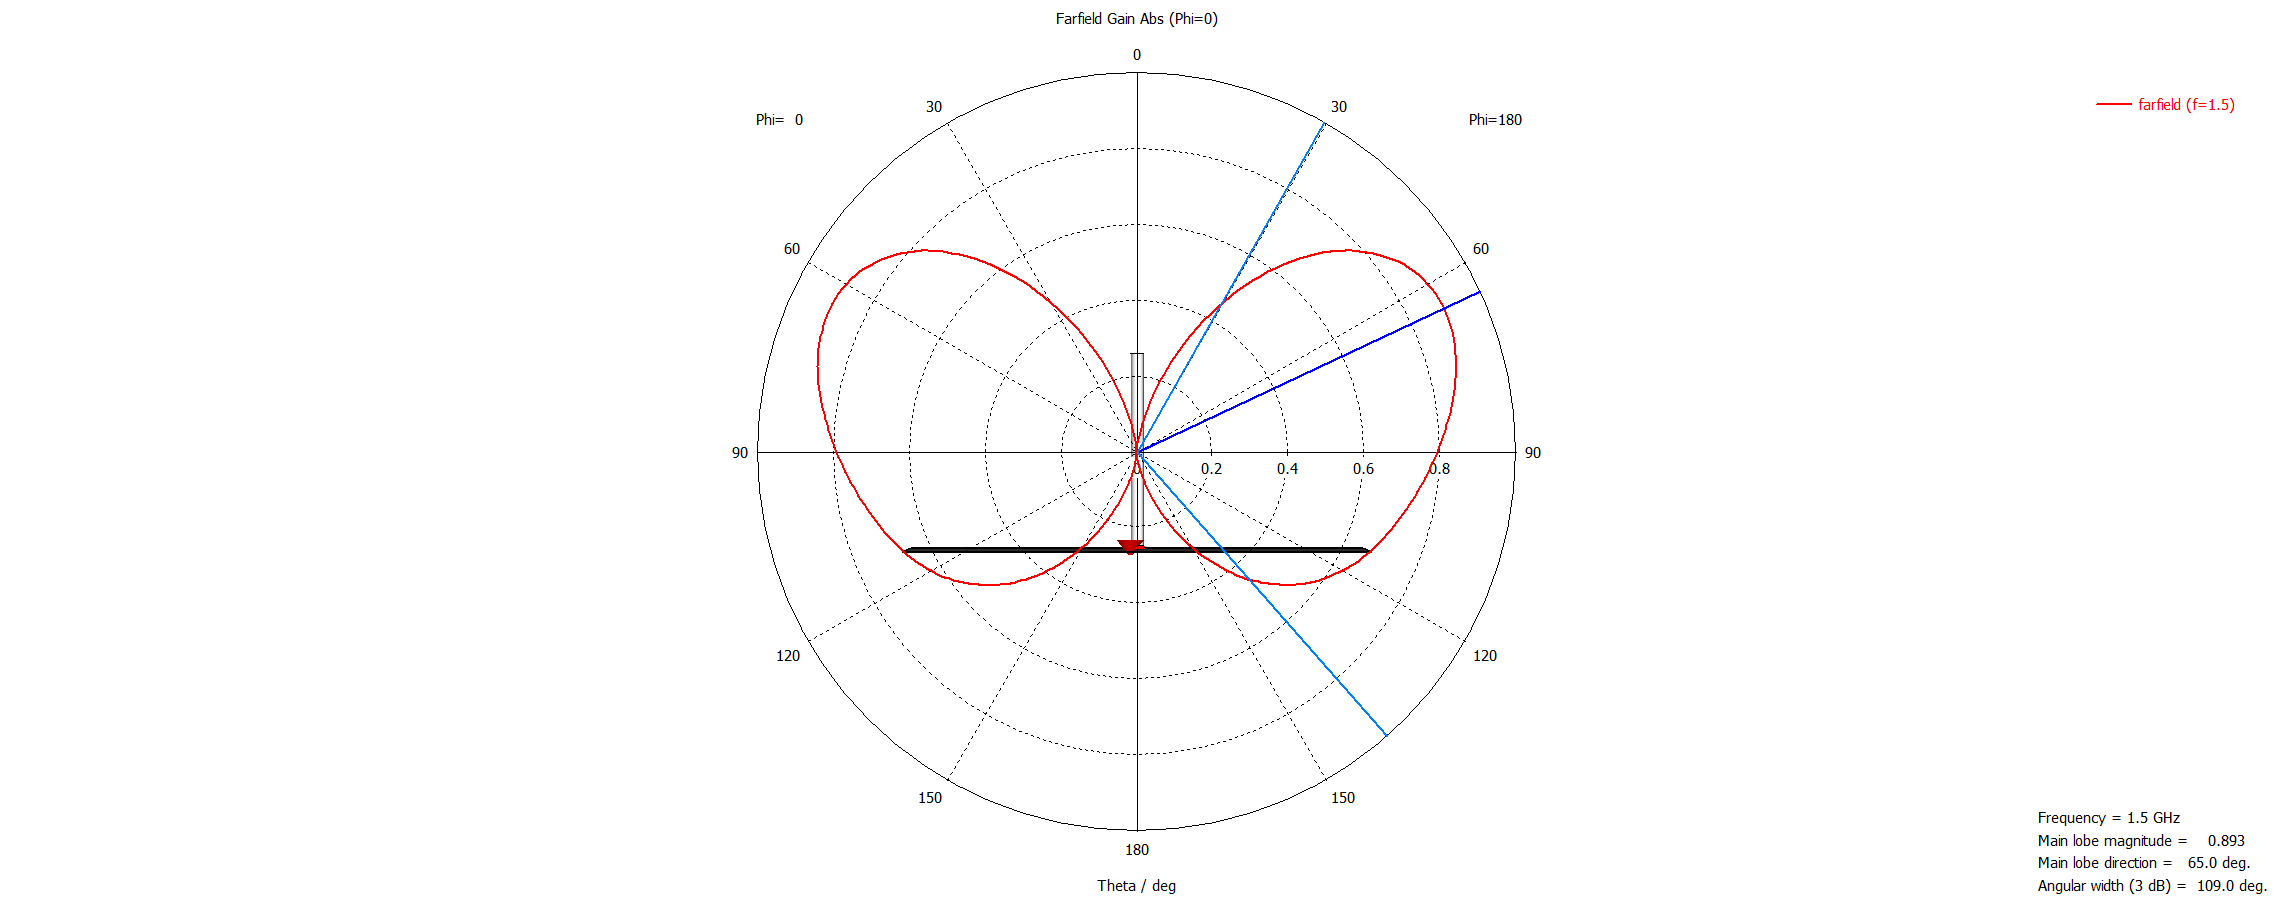
\includegraphics[width=14cm,valign=c]{Images/qw-farfield-plot-xz-plane.png}
	\caption{The monopole's far-field in 2D shown from the X-Z plane}  %% Caption for your figure
	\label{fig:qw_ff_2d}
\end{figure}


\end{document}
